\documentclass{beamer}
\usetheme{afm}

\title{Interest Rate Derivatives}
\subtitle{Main Ineterst Rate Contracts Theory}
\course{Advanced Financial Modelling}
\author{\href{mailto:matteo.sani@unisi.it}{Matteo Sani}}

\begin{document}
\begin{frame}[plain]
  \maketitle
\end{frame}

\section{Numerical Algorithms}
\subsection{Root Finding Methods}
\begin{frame}[fragile]{Newton-Raphson Method}
	\begin{itemize}
		\item The roots of the function (or zeros) are the $x_i$ solutions of $f(x) = 0$.
		\item \emph{Newton's method} is a root-finding algorithm which produces successively better approximations of the roots.
		\item Start with an initial guess $x_0$, approximate the function by its tangent line $g(x)$, and compute the $x$-intercept of this line
		\begin{gather*}
			g(x) = f(x_0) + f'(x_0)(x-x_0) \implies  f'(x_0)(x_0-x_1)=f(x_0)\\
			x_1=x_0-\frac {f(x_0)}{f'(x_0)}
		\end{gather*}
		%\item This $x$-intercept will typically be a better approximation to the original function's root than the first guess, and the method can be iterated.
		\item If the tangent line to the curve $f(x)$ at $x = x_0$ intercepts the $x$-axis at $x_{1}$ then
		\begin{equation*}
			\begin{cases}
				f(x_1) < \text{tol}=10^{-8} \Rightarrow \text{ zero found !}\\
				g(x_1) = f(x_0) + f^{'}(x_0)(x_1-x_0) = 0 \Rightarrow \text{ solve for
				}x_1\text{ and iterate...}
			\end{cases}
		\end{equation*}
		\item The method will usually converge, provided this initial guess is close enough to the unknown zero, and that $f'(x_0) \neq 0$.
	\end{itemize}
\end{frame}

\begin{frame}[fragile]{Newton-Raphson Method}
\begin{center}
    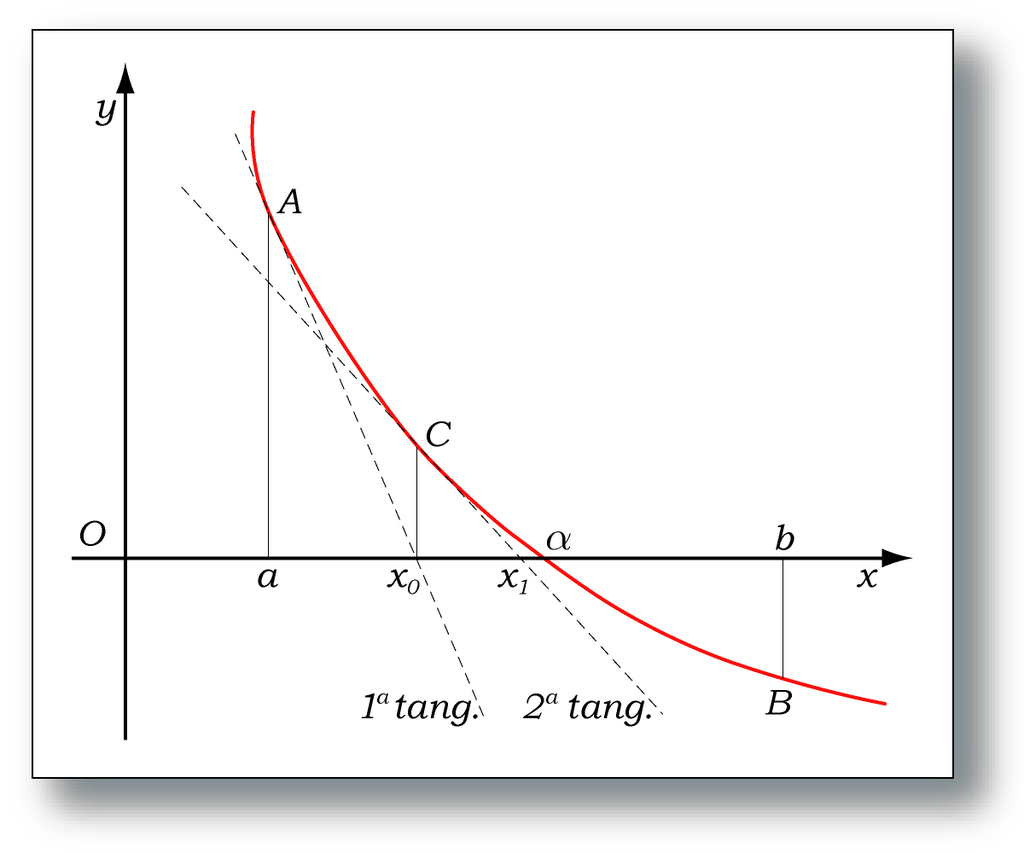
\includegraphics[width=0.6\linewidth]{images/newton_raphson}
\end{center}
\end{frame}

\subsection{Bootstrap}
\begin{frame}{Bootstrapping the Interest Rate Curve}
\begin{itemize}
\item A \emph{yield curve} shows the relationship between interest rates and the time to maturity of the debt.
\item Market instruments like swaps have different maturities and coupon structures.
\item \textbf{Bootstrapping} is a technique to derive the zero-coupon yield curve from these market prices.
\item Swap rates reflect market expectations of future interest rates, making them crucial for yield curve construction.
\end{itemize}
\end{frame}

\begin{frame}{The Bootstrapping Methodology}
\begin{itemize}
\item Gather market data for interest rate swaps with various maturities. Each swap provides a fixed rate (swap rate) and a set of cash flows
\begin{equation*}
\textbf{RFS} = N\sum_{i=\alpha+1}^{\beta}\tau_i P(t,T_i)(K-F(t;T_{i-1},T_i))
\end{equation*}
\item Start with the shortest maturity instrument (e.g. 1M swap with 1 month tenor)
\begin{equation*}
\textbf{RFS}_{1M} = N\tau_{01} (K-F_{01})
\end{equation*}
Since at inception its value is $\textbf{RFS}_{1M} = 0$, using Newton-Raphson calculate the corresponding zero-coupon rate for this maturity
\begin{equation*}
\textbf{RFS}_{1M} = N\tau_{01} (K-F_{01}(\textcolor{green}{r_0}, \textcolor{red}{r_1})) = 0
\end{equation*}
\end{itemize}
\end{frame}

\begin{frame}{The Bootstrapping Methodology}
\begin{itemize}
\item Move to the next maturity
\begin{equation*}
\textbf{RFS}_{2M} = N\tau_{01} (K-F_{01}) + N\tau_{12} (K-F_{12})
\end{equation*}
\item Use the known zero-coupon rates from the shorter maturities to determine the zero-coupon rate for this maturity such that the present value of all cash flows equals the swap's par value
\begin{equation*}
\textbf{RFS}_{2M} = N\tau_{01} (K-F_{01}(\textcolor{green}{r_0}, \textcolor{green}{r_1})) + N\tau_{12} (K-F_{12}(\textcolor{green}{r_1}, \textcolor{red}{r_2})) = 0
\end{equation*}
\item Repeat the process, step-by-step, for each successive maturity, using previously calculated zero-coupon rates.
\item This process "bootstraps" the yield curve, building it from the short end to the long end.
\end{itemize}
\end{frame}

\begin{frame}{Bootstrapping from Interest Rate Swaps: An Example}
\begin{center}
    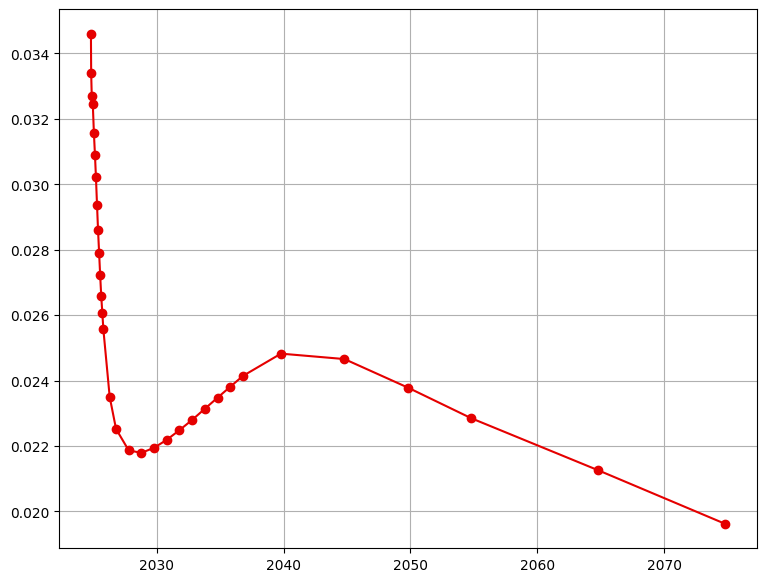
\includegraphics[width=0.6\linewidth]{images/forward_rate_curve}
\end{center}
\end{frame}

\section{Risk Measures}
\begin{frame}{Sensitivity}
\begin{itemize}
\item The assignment of the correct price to a derivative is not the whole story.
\item \emph{Sensitivity} measures how much the value of a financial instrument changes in response to a change in an underlying factor.  
\item Understanding sensitivity helps investors to:
\begin{itemize}
    \item \emph{Assess Risk:} identify potential vulnerabilities and understand how different market movements can impact portfolio value;
    \item \emph{Manage Portfolios:} make informed decisions about asset allocation and hedging strategies to optimize risk-return profiles;
    \item \emph{Compare Investments:} evaluate the relative risk and potential reward of different investments based on their sensitivities.
\end{itemize}
\item The sensitivity concept closely resamble the mathematical definition of \emph{derivative}, so in the very end estimating the sensitivity is as simple as computing a ratio of variations.
\end{itemize}
\end{frame}

%\begin{frame}{Sensitivity}
%There are several metrics to estimate the risk and different ways to measure its actual value:
%\begin{itemize}
%\item \textbf{Duration:} measures a bond's sensitivity to changes in interest rates (higher duration greater price change for a given interest rate shift)
%\begin{equation*}
%D(y)\equiv -\cfrac{1}{P}\cdot \cfrac{\partial P}{\partial y}=-\cfrac {\partial \ln(P)}{\partial y}\quad\text{ definition as derivative}
%\end{equation*}
%Its interpreation as sensitivity of a bond's market price to interest rate (i.e. yield) movements comes from
%\begin{equation*}
%D\approx -\cfrac {1}{P}\cfrac{\Delta P}{\Delta y}\rightarrow \Delta P\approx -P\cdot D\cdot \Delta y
%\end{equation*}
%Thus duration is approximately equal to the percentage change in price for a given finite change in yield.
%\item \textbf{Beta:} measures a stock's sensitivity to changes in the overall market ($\beta > 1$ indicates higher volatility than market).
%\item \textbf{Delta:} measures an option's sensitivity to changes in the price of the underlying asset.
%\end{itemize}
%\end{frame}

\begin{frame}{Sensitivity Calculation}
Sensitivities can be computed with different techniques:
\begin{itemize}
	\item \textbf{analytical}: involves deriving a closed-form expression which can be complex (and not always feasible);
	\item \textbf{numerical}: one bumps the yield curve calibration instruments and reprice the derivative. The change in price gives the risk;
%	\item \textbf{curve Jacobians}: when yield curves have been calibrated, the solver slope 'Jacobian' can be kept and used to give the change in derivative price for a change in forwards/discount factors;
	\item \textbf{algorithmic differentiation}: can be used to compute risk "automatically" at the same time as computing the price. It produces accurate and fast risk estimates.
\end{itemize}
\end{frame}

\begin{frame}{Sensitivity in IRD World}
\begin{itemize}
\item<1-> The concept of risk on interest rate derivatives measures precisely the risk associated with the shift of the interest rate curve. 
\item<2-> However there are a number of complications...
\item<2-> Interest rate derivatives depend on a variety of instruments, used in the determination of the interest rate curve, rather than a single asset.
\item<3-> Because there are many ways of shifting the interest rate curve, many different deltas can be computed. 
\end{itemize}
\end{frame}

\begin{frame}{PV01}
\begin{itemize}
    \item<1-> \textcolor{red}{PV01} refers to present value of 1 basis point and it's the discounted value of the cashflows for a rate of 0.01\% for all periods of a particular instrument, (i.e. the NPV of the fixed leg with a rate of 0.01\%).
	\begin{equation}
	   \textbf{PV01} = 0.01\% \frac{\partial \textbf{PFS}}{\partial K} = 0.01\% \sum_{i=\alpha+1}^\beta\tau_iP(t,T_i)
	\end{equation}
	\item<2-> This is a useful measure for dealers calculating the exact P\&L generated by applying a spread (or margin) to a fixed rate away from the mid-market rate.
   \item<3-> Besides giving you the information on how a currency amount would affect the fixed rate (incorporate a fee for example), the PV01 is not useful as a risk measure. 
\end{itemize}
\end{frame}

\begin{frame}{DV01}
\begin{itemize}
	\item<1-> \textcolor{red}{DV01} refers to dollar (actually currency amount) value of 1 basis point and it's the change in value of the NPV of the instrument with a change of 1 basis point in the curve(s). The average of the change for -1bp and +1bp to be more precise. 
	\item<2-> You can consider what happens to the NPV if every rate $r_i$ is changed in parallel by the same amount
	\begin{equation*}
	\textbf{DV01} = \sum_j \frac{\partial \textbf{PFS}}{\partial r_j} = -\sum_{j}\tau_jP_j+\sum_{j}\left(K\sum_{i=\alpha+1}^\beta\tau_i\frac{\partial P_i}{\partial r_j} - \sum_{k=\alpha+1}^\beta L_k\tau_k\frac{\partial P_k}{\partial r_j}\right)
	\end{equation*}
	\item<3-> In the multi-curve framework DV01 would be calculated for the forecast curve, and for the discounting curve, resulting in two actual DV01 measurements.
    \item<4-> When the swap is at fair value (NPV = 0), PV01 and DV01 are very very close although not exactly the same, otherwise they will be different.
    %\item<5-> For given set of market data, changing the swap rate will not change the PV01 but will change the DV01.
    \item<5-> A trader care mostly about DV01 (as a number or, better yet, divided into buckets) because wants to know how the P\&L changes if the curves change by 1bps.
\end{itemize}
\end{frame}

\begin{frame}{DV01 Numerical Calculation}
\begin{itemize}
	\item<1-> Assume the P\&L on a Swap could be approximated with a linear term plus its convexity
	\begin{equation*}
	\Delta \textbf{PFS}(\delta r)\approx \frac{\partial \textbf{PFS} }{\partial r}\delta r + \frac{1}{2}\frac{\partial^2 \textbf{PFS}}{\partial r^2}\delta r^2
	\end{equation*}
	\item<2-> Then bumping $\delta r$ by $\pm 1$~bp and dividing by 2 eliminates the convexity element and very accurately approximates the DV01
	\begin{equation*}
	\textbf{DV01} = \frac{\Delta \textbf{PFS}(+1~bp)-\Delta \textbf{PFS}(-1~bp)}{2}=\frac{\partial \textbf{PFS} }{\partial r}
	\end{equation*}
	\item<3-> Another common method of calculation is to use a single bumped curve by, say, $\frac{1}{100}$th of a bp, and scale the result by 100 (less accurate, since the convexity is marginalised and not eliminated)
	\begin{equation*}
	100\Delta \textbf{PFS}\left(\frac{1}{100}~bp\right)=\frac{\partial \textbf{PFS}}{\partial r}+\frac{1}{200}\frac{\partial^2\textbf{PFS}}{\partial r^2}
	\end{equation*}
	\end{itemize}
\end{frame}

\begin{frame}{Market Rate Sensitivity}
\begin{itemize}
	\item<1-> Forecast and discount curves used in pricing formulas are those \emph{implied} by the market quotes of interest rate instruments (i.e. futures, OIS, etc\ldots). They are usually determined through the \textbf{bootstrap} technique.
	\item<2-> Another popular, though more complicated, method to assess the risk is to shock each input instrument used in the bootstrapping by 1~bp one by one, rebuild the curves, and then re-price the instrument of interest to obtain its curve sensitivity. 
	\item<3-> This is called \textcolor{red}{Market Rate Sensitivity} and its value is given by the sum of each Swap $NPV$ variations.
	\item<4-> This of course is not quite a "parallel" shift of any curve (e.g. a 1~bp change in futures rate won't correspond to a 1~bp change in the others).
\end{itemize}
\end{frame}

%\begin{frame}{Market Rate Sensitivity}
%In a plain vanilla Swap is very close but not equal to DV01. The mark to market value of the Swap is \textcolor{red}{not linear} (as in a future contract), but rather it is a \textcolor{red}{convex} function of the rates (just like a bond is a convex function of the yield).
%\begin{center}
%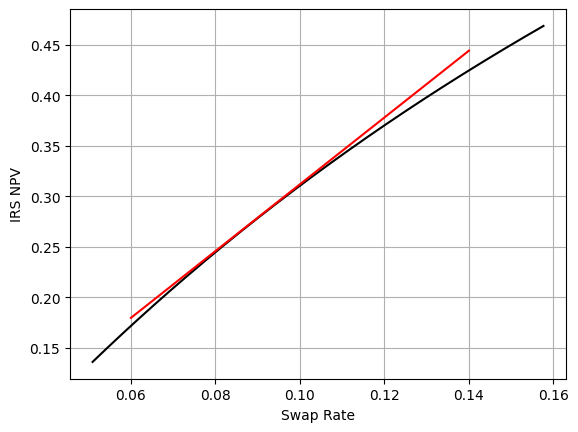
\includegraphics[width=0.5\linewidth]{images/dv01}
%\end{center}
%\end{frame}

\begin{frame}[fragile]{Algorithmic Differentiation}
Consider the following function
\begin{equation*}
\begin{cases}
\text{Function: } f(x_0, x_1) = 2x_0^2 + 3x_1\\
\text{Solution: } \frac{df}{dx_0} = 4x_0, \text{ and } \frac{df}{dx_1}=3
\end{cases}
\end{equation*}
\begin{columns}
\column{0.4\linewidth}
Let's try to compute its derivative by explicitly defining the $f'$ and using the adjoint technique, when $x_0=2$ and $x_1=3$,

\begin{equation*}
\frac{df}{dx_0} = 8, \text{ and } \frac{df}{dx_1}=3
\end{equation*}
\column{0.6\linewidth}
\begin{ipython}
import numpy as np, tensorflow as tf

def f(x):
  return 2*x[0]**2+3*x[1]

def df_tangent(x):
  return 4*x[0], 3

def df_adjoint(x):
  x = tf.Variable(x, dtype='float', name='x')
  with tf.GradientTape() as tape:
    f = 2*x[0]**2+3*x[1]
  return tape.gradient(f, x)

x = (2, 3)
print (df_tangent(x), df_adjoint(x))
\end{ipython}
\begin{ioutput}

(8, 3) tf.Tensor([8. 3.], shape=(2,), dtype=float32)
\end{ioutput}
\end{columns}
\end{frame}

\begin{frame}[fragile]{Algorithmic Differentiation Example}
Compute DV01 for a 5-years receiver IRS with a 1M notional, exchanging a fixed rate of 5\% with a flat 1\% EURIBOR rate with annual payments.

The explicit derivative is
\begin{equation*}
\begin{gathered}
\cfrac{\partial PV_{float}}{\partial r_i} = \cfrac{\partial}{\partial r_i}\sum_j N\tau F_j e^{-r_j t_j} = \sum_j N\tau \cfrac{\partial F_j}{\partial r_i} e^{-r_j t_j} - F_i t_i e^{-r_i t_i} \\
\cfrac{\partial PV_{fix}}{\partial r_i} = \cfrac{\partial}{\partial r_i}\sum_i N\tau K e^{-r_i t_i} = - N\tau K t_i e^{-rt_i}        
\end{gathered}
\end{equation*}
\end{frame}

\begin{frame}[fragile]{Algorithmic Differentiation Example}
\begin{columns}
\column{0.5\linewidth}
\begin{ipython}
import numpy as np
import tensorflow as tf

class Swap:
  def __init__(self, notional, fixed_rate, tau, terms, rates):
    self.N = notional; self.K = fixed_rate
    self.tau = tau; self.t = terms
    self.r = tf.Variable(rates, name="rates", dtype=tf.float64)

  def swap_price(self, dr=0.0001):
    fixed_pv = tf.Variable(0.0, dtype=tf.float64)
    float_pv = tf.Variable(0.0, dtype=tf.float64)

    with tf.GradientTape(persistent=True) as tape:
      for i in range(1, len(self.t)):
        fixed_pv = fixed_pv + self.K*self.tau
                   *tf.math.exp(-self.r[i]*self.t[i])
      for j in range(1, len(self.terms)):
        F = (self.r[j]*self.t[j]-self.r[j-1]*self.t[j-1])
        float_pv = float_pv + F*tf.math.exp(-self.r[j]*self.t[j])
    
    fixed_pv_dot = np.sum(dr*tape.gradient(fixed_pv, self.r))
    float_pv_dot = np.sum(dr*tape.gradient(float_pv, self.r))

    swap_pv = self.N*(fixed_pv - float_pv)
    swap_pv_dot = self.N*(fixed_pv_dot - float_pv_dot)

    return swap_pv, swap_pv_dot
\end{ipython}
\column{0.5\linewidth}
\begin{ipython}
N = 1e6
fixed_rate  = 0.015
tau         = 1.0
terms       = np.array([0.0, 1.0, 2.0, 3.0, 4.0, 5.0])
rates       = np.array([0.01, 0.012, 0.013, 0.014, 0.016, 0.017])

swap = Swap(N, fixed_rate, tau, terms, rates)
price, dv01 = swap.swap_price()

print (f"Swap price: {price:,.2f}")
print (f"DV01: {dv01:,.2f}")
\end{ipython}
\begin{ioutput}

Swap price: -9,097.43
DV01: -472.60
\end{ioutput}
\end{columns}
\end{frame}

%https://quant.stackexchange.com/questions/49582/interest-rate-swap-pv01-vs-dv01
%https://quant.stackexchange.com/questions/70346/fixed-vs-float-swap-interest-rate-risk/70426#70426
%https://math.nyu.edu/~avellane/DerivativeSecurities7.pdf

%1) Why does an interest rate swap have no duration, but it does have a DV01?

%Every spread product has duration and DV01 since all are sensitive to underlying moves in rates. To calc duration on a swap it's your notional/DV01 * 10k. As your swap reaches maturity the duration and DV01 factors down. Longer duration swaps, say 10Y vs 2Y, will inherently have more duration. Ex. a 10Y swap will have a duration slightly less than 10 depending on how much time to maturity left on the position.  
%
%For 2 and 3, do not think of each leg of the swap having DV01. Rather, the entire swap itself (both legs) is one position with DV01 depending on if you are paying/receiving fixed vs float.
%
%2) What does it mean for the fixed leg of an interest rate swap to have positive DV01?
%
%If you pay fixed and receive float, the entire swap has a positive DV01. Rates sell off (go higher), and you receive positive PnL on the position = positive DV01.


%%\begin{frame}{Trading and Hedging Swaps}
%%	For example, the yield spread is 0.6524\%. An investor believes that this yield spread will narrow as inter-bank credit improves relative to German Sovereign credit. By entering into a position which profits from a rise in the lower (German	Sovereign) yields and / or a fall in the higher (inter-bank) yields, the investor is able to express his view on relative credit pricing.
%%	AGGIUNGERE UN PO' DI SPIEGAZIONE
%%\end{frame}

\begin{homework}
\begin{frame}{\textcolor{white}{Homework}}
\begin{itemize}
\item[white] Consider a 2-year Interest Rate Swap on a notional of 1M, with a fixed rate of 5\% and paying Libor rate annually. The term-structure of interest rates is flat at 5\%.
Estimate the DV01 of the swap numerically.  
\end{itemize}
\end{frame}
\end{homework}

\section{Cap and Floor}
\begin{frame}{Caps and Floors}
	\begin{itemize}
		\item<1-> A \textcolor{red}{Cap} is a Payer IRS in which the payment is done only if the payoff is positive. Its value is the expectation of 
		\begin{equation}
			\sum_{i=\alpha+1}^{\beta}D(t,T_i)N\tau_i\max\left[L(T_{i-1},T_i)-K,0\right]
			\label{eq:cap}
		\end{equation} 
		\item<2-> The cap allows investors which have a debt at a variable rate to buy insurance against high rates in the future.
		\item<3-> A \textcolor{red}{Floor} is the same kind of object but analogous to a Receiver IRS:
		\begin{equation}
			\sum_{i=\alpha+1}^{\beta}D(t,T_i)N\tau_i\max\left[K-L(T_{i-1},T_i),0\right]
			\label{eq:floor}
		\end{equation} 
	\end{itemize}
\end{frame}

\subsection{Caplets}
\begin{frame}{Caplet and Floorlet}
	\begin{itemize}
		\item<1-> Considering each element of the sum in \cref{eq:cap} or \cref{eq:floor} we see that Cap/Floor can be split into forward starting options over a floating rate, called \textcolor{red}{Caplet/Floorlet}.
		\item<2-> A Caplet/Floorlet payoff is defined as
		\begin{equation*}
			D(t,T_i)N\tau_i\max\left[L(T_{i-1},T_i)-K,0\right]
		\end{equation*} 
		and its value is given by
		\begin{equation}
			\textbf{Cpl}(t,T_{i-1},T_i,\tau,N,K)=\expect{Q}\left[e^{-\int_t^{T_i}r_s ds}N\tau(L(T_{i-1},T_i)-K)^+ | \mathcal{F}_t\right]
		\end{equation}
		\item<3-> This can also be written
		\begin{equation*}
			\textbf{Cpl}=N\expect{Q}\left[e^{-\int_t^{T_{i-1}}r_s ds}\tau P(T_{i-1},T_i)(L(T_{i-1},T_i)-K)^+ | \mathcal{F}_t\right]
		\end{equation*}
	\end{itemize}
\end{frame}

\begin{frame}{Caplets as ZCB Options}
	\begin{itemize}
		\item<1-> Using the LIBOR rate definition we get
		\begin{equation*}
			\begin{aligned}
				\textbf{Cpl} &=N\expect{Q}\left[e^{-\int_t^{T_{i-1}}r_s ds}P(T_{i-1},T_i)\left(\frac{1}{P(T_{i-1},T_i)}-1-K\tau\right)^+ \Big\rvert \mathcal{F}_t\right] \\
				& = N\expect{Q}\left[e^{-\int_t^{T_{i-1}}r_s ds}\left(1-(1+K\tau)P(T_{i-1},T_i)\right)^+ | \mathcal{F}_t\right]
			\end{aligned}
		\end{equation*}
		\item<2-> Collecting ($1+K\tau$) we finally get
		\begin{equation}
			\boxed{\textbf{Cpl}=N(1+K\tau)\expect{Q}\left[e^{-\int_t^{T_{i-1}}r_s ds}\left(\frac{1}{1+K\tau}-P(T_{i-1},T_i)\right)^+ \Big\rvert \mathcal{F}_t\right]}
		\end{equation}
	\end{itemize}
\end{frame}

\begin{frame}{Caplets as ZCB Options}
	\begin{block}{Intepretation}
		\begin{enumerate}
		\item Caplets can be seen as \textcolor{red}{put options} on ZCBs
\begin{equation*}
\textbf{Cpl}=N'\expect{Q}\left[D(t,T_{i-1})\left(K'-P(T_{i-1},T_i)\right)^+ \Big\rvert \mathcal{F}_t\right]
\end{equation*}
		\item Similarly floorlets are \textcolor{red}{call options} on ZCBs
\begin{equation}
\textbf{Flr}=N'\expect{Q}\left[D(t, T_{i-1})\left(P(T_{i-1},T_i)-K'\right)^+ \Big\rvert \mathcal{F}_t\right]
\end{equation}
		\end{enumerate}
	\end{block}
\end{frame}

\section{Swaptions}
\begin{frame}{Swaptions Overview}
\begin{itemize}
	\item<1-> The purchaser of an \textcolor{red}{European swaption} has the right but not the obligation to enter into a swap contract, at a given future time, called the \textcolor{red}{swaption maturity}.
	\item<2-> There are two types of \textcolor{red}{swaptions} (as the underlying swaps): a \emph{payer} in which at maturity the buyer could become the fixed-rate payer and a \emph{receiver} where she could become the fixed-rate receiver.
	\item <3-> The strike price of the swaption determines the fixed rate of the underlying swap.
	\item<4-> A swaption provides protection for a borrower as it ensures a maximum fixed interest rate payable in the future. Furthermore, it gives her the flexibility, if the rate does not rise above the swaption strike rate at expiry, to choose not to exercise it and take advantage of the lower market rates.
\end{itemize}
\end{frame}

\begin{frame}{Swaptions Overview}
	\begin{itemize}
	\item<1-> Usually, the swaption maturity coincides with the first reset date of the underlying IRS (the Interest Rate Swap length is called the \textcolor{red}{tenor} of the swaption).	
	\item<2-> If you are on the buyer side (you are long payer swaption) which is your view on rates ? Why ?
	\item<2-> Are there any risks associated with a Swaption?
	\begin{itemize}
		\item<3-> The primary risk with a Swaption occurs after you have exercised your right and proceeded with the Swap. Should interest rate movements be different to your expectations, the Swap may have the opposite effect to what you were trying to achieve with the transaction. 
		\item<3-> If interest rates do not rise above the strike on the exercise date, you have not obtained any benefit from the premium paid for the purchase of the Swaption. The premium is the cost of obtaining protection against a rise in interest rates.
	\end{itemize}
\end{itemize}
\end{frame}

\begin{frame}{Swaption Payoff}
\begin{itemize}
	\item<1-> The discounted payoff of a payer Swaption (with maturity $T_\alpha$) is given, recalling the value of a payer IRS by % (\cref{eq:swap_as_sum_fra}) by
	\begin{equation}
		\textbf{PSw}=D(t,T_\alpha)\left(\sum_{i=\alpha+1}^\beta P(T_\alpha,T_i)\tau_i (F(T_\alpha;T_{i-1},T_i) - K)\right)^+
		\label{eq:swaption_payoff_std}
	\end{equation}
	\item<2-> Unfortunately this payoff \textcolor{red}{cannot} be easily decomposed into elementary parts (as done for Cap/Floor). Indeed the \emph{positive part operator} $(\cdot)^+$ is "outside" the summation (while for Caps it is "inside").
	\item<3-> Nevertheless it can be simplified by writing it in a different way...
	%		\begin{equation}
		%			ND(t,T_\alpha)\left(S_{\alpha,\beta}(T_\alpha)-K\right)^+\sum_{i=\alpha+1}^\beta \tau_i P(t,T_i)
		%		\end{equation}
\end{itemize}
\end{frame}

\begin{frame}{Swaption Payoff}
\begin{itemize}
	\item<1-> Recall that we have expressed the swap payoff also as %(\cref{eq:swap_payoff_with_swap_rate})
	\begin{equation*}
	\textbf{PFS}=\sum_{i=\alpha+1}^\beta \tau_i P(t,T_i)(S_{\alpha,\beta}-K) = A(S_{\alpha,\beta}-K)
	\end{equation*}
	\item<2-> If we look at the swaption payoff through this expression modeling as stochastic variable directly $S_{\alpha,\beta}(t)$, instead of each forward rate $F(t;T_{i-1},T_i)$, we can write the swaption price as the expectation of
	\begin{equation}
		\boxed{\textbf{PSw}=\expect{Q}\left[D(t,T_\alpha)A (S_{\alpha,\beta}(T_\alpha)-K)^+\right]}
	\end{equation}
	which looks like easier and more intuitive than previous \cref{eq:swaption_payoff_std}.
\end{itemize}
\end{frame}

\begin{frame}{Swaption Characterization}
	\begin{itemize}	
		\item We characterize the payoff in three different ways
		\begin{enumerate}
			\item The swaption is said to be \textcolor{red}{at-the-money} (ATM) if
			\begin{equation*}
				K = K_{ATM} = S_{\alpha,\beta}(0) = \frac{P(0,T_\alpha)-P(0,T_\beta)}{\sum_{i=\alpha+1}^\beta \tau_i P(0,T_i)}
			\end{equation*}
			where $T_\alpha$ is the maturity of the swaption, and $T_\beta$ the last payment date of the underlying swap (the first being $T_{\alpha+1})$. That is when the strike is equal to the swap forward rate $S_{\alpha,\beta}$.
			\item The payer swaption is \textcolor{red}{in-the-money} if $K<K_{ATM}$ and \textcolor{red}{out-of-the-money} otherwise.
			\item The opposite holds for the receiver swaption.
		\end{enumerate}
		\item ATM swaptions are quoted for maturities ranging between $1m$ and $30y$, and for tenors between $1y$ and $30y$.
	\end{itemize}
\end{frame}

%\begin{frame}{Swaption as an Option on a Swap}
%	\begin{itemize}
%		\item So the forward rates are the chosen state variable, also the correlation between them is needed...
%		\item Market practice: approximation formula (see chapter 6 of Brigo-Mercurio) the definitive reference for this issue.
%		\item Clearly here a model which accounts for terminal correlations needed.
%		\item Which is the relationship between a Cap and a payer swaption with the same payment and roll dates ?
%	\end{itemize}
%
%\end{frame}

\begin{frame}{An Example}
	\begin{itemize}
		\item \textbf{A} has raised a $10y$ loan with floating interest rates fixed every three months (IBOR + margin).
		\item \textbf{A} wants to \emph{hedge the loan against rising interest rates but also to benefit from the floating rate}, i.e. should interest rates not rise above a certain level (the swaptions strike-rate $K$).
		\item The purchase of a payer swaption could hedge this risk: 
		\begin{columns}
			\column{0.45\linewidth}
			\begin{itemize}
				\item \textbf{interest rates increase}: \textbf{A} may exercise the swaption and be a party of a swap as a payer of a fixed interest rate;
				\item \textbf{swap-rate below $K$}: it will not be exercised and \textbf{A} will continue to have floating-rate funding.
			\end{itemize}
			\column{0.45\linewidth}
			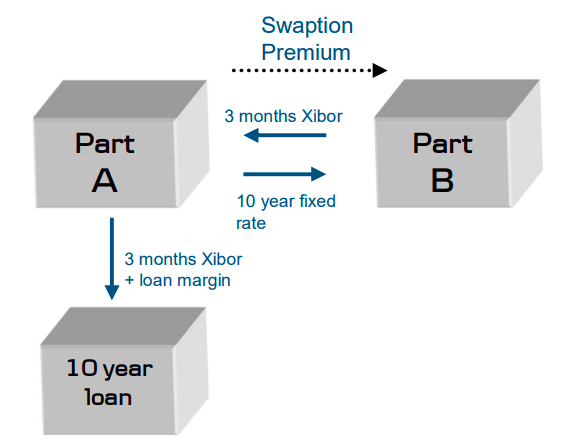
\includegraphics[width=1.\linewidth]{images/swaption_example}
		\end{columns}
	\end{itemize}
\end{frame}

\begin{homework}
\begin{frame}{\textcolor{white}{Homework}}
\begin{itemize}
\item[white] In order to hedge your position against interest rate movements which kind of contract would you use: 
\begin{itemize}
\item[white] a Swap
\item[white] a Cap/Floor
\item[white] a Swaption
\end{itemize}
List the pros and cons about each one and declare your favourite.
\end{itemize}
\end{frame}
\end{homework}

\section{The Black Model}
\begin{frame}{The Black Model - Overview}
	\begin{itemize}
		\item The \textcolor{red}{Black Model} extends the Black-Scholes formula to \emph{caplets} and \emph{swaptions}. % and \emph{bond options}. %It uses the forward coordinates, not the spot ones; this last is not a minor issue indeed.
		\item The main difference with respect to the Black-Scholes set up is that \textcolor{red}{forward rates $F(t;T_{i-1},T_i)$ (or swap rates $S_{\alpha\beta}(t)$) are log-normally distributed}, rather than the spot price of the underlying. 
		\item It should be stated that Black’s formulas did not originally correspond to prices that arise from the application of martingale pricing theory to some particular model. 
		\item The advent of the \emph{market models} will provide a belated justification for these formulas but we shall see that the justifications are mutually inconsistent. 
		\item Indeed, it may be shown that if forward rates have deterministic volatilities then it is not possible for swap rates to also have deterministic volatilities. Therefore Black’s formulas for caplets and swaptions cannot both hold within the same model. 
	\end{itemize}
\end{frame}

%\begin{frame}{The Black Model: Overview}
%	\begin{itemize}
	%		\item It should be recognized that the Black model is being actually used in different ways. In particular the caps uses the forward short-term LIBOR rate as the underlying state variable, whereas the swaptions uses longer-term forward swap rates. Beause forward swap rates are nearly linera in individual forward rates , the lognormality assumption implicit in the Black model cannot hold simultaneously for both, since a linear combination of lognormal variables is not lognormal.
	%	\end{itemize}
%\end{frame}

%\begin{frame}{The Black Model: Overview}
%	\begin{itemize}
	%	\item It should be stated that Black’s formulae for caps and swaptions did not originally correspond to prices that arisefrom the application of martingale pricing theory to some particular model. 
	%	\item It is widely used in practice as the metric by which traders translated volatilities into prices until rates became too low and the model collapsed under the assumption of positive rates.
	%		\item 
	%		\item ...but for the moment we cannot consider it as a model ! Just a bunch of formulas.
	%		
	%
	%
	%When we model swap rates directly as in (30) we say that we have a swap market model. Thiscontrasts with the LIBOR market models of Section 4.Remark 5 The advantage of Black’s swaption formula is that it is elegant and exact, whereas the BGM formula is cumbersome and only an approximation. However, the BGM approximation is consistent with Black’s formulae for caplets and caps whereas Black’s swaption formula is not. 
	%That said, within the LIBOR market framework with deterministic volatilities, it can be argued thatforward swap rates are approximately log-normally distributed.
	%
	%
	%	\end{itemize}
%\end{frame}

\begin{frame}{Pricing Caps with the Black-76 Formula}
	\begin{block}{Definition}
		\begin{equation}
			\begin{aligned}
				\textbf{Cap}_{Bl}(0, \tau,N,K,\sigma_{\alpha,\beta}) &= N\sum_{i=\alpha+1}^{\beta}\textbf{Cpl}_{Bl}(T_i, \tau,K,\sigma_{\alpha,\beta}) = \\ &=N\sum_{i=\alpha+1}^{\beta}\tau P(0,T_i) \textbf{Bl}(K,F(0;T_{i-1},T_i),v_i)
			\end{aligned}
			\label{eq:cap_black}
		\end{equation}
		where
		\begin{equation*}
			\begin{gathered}
				\boxed{\textbf{Bl}(K,F_i,v_i)=F\Phi(d_1(K,F_i,v_i)) - K\Phi(d_2(K,F_i,v_i))} \\
				d_{1,2} = \frac{\log{\cfrac{F_i}{K}} \pm \cfrac{v_i^2}{2}}{2} \\[0.2cm]
				v_i = \sigma_{\alpha,\beta}\sqrt{T_{i-1}}
			\end{gathered}
		\end{equation*}
	\end{block}
\end{frame}

\begin{frame}{Black Formula for Swaptions}
	\begin{itemize}
		\item The most common way to price European Swaption is through the Black formula.
		\item Replacing the forward rate $F(0;t_{i-1},t_i)$ with the swap rate $S_{\alpha,\beta}(0)$ and plugging in the quoted swaption volatility you get Black's formula for swaptions
		\begin{equation}
			\boxed{\begin{aligned}
					\textbf{PSw}_{Bl}(0,T,&N,K,S_{\alpha,\beta})=\\
					&N\left[S_{\alpha,\beta}(0)\Phi(d_1)-K\Phi(d_2)\right]\sum_{i=\alpha+1}^\beta P(0,T_i)\tau_i
			\end{aligned}}
		\end{equation}
		where
		\begin{equation*}
			\begin{gathered}
				d_{1,2} = \cfrac{\log{\frac{S_{\alpha,\beta}}{K}} \pm \frac{v^2}{2}}{2}\\[0.2cm] 
				v = \sigma_{\alpha,\beta}\sqrt{T_\alpha}
			\end{gathered}
		\end{equation*}
	\end{itemize}
\end{frame}

\begin{frame}[fragile]{Newton-Raphson Application}
	Using the Newton-Raphson method determine the implied volatility of a \textbf{call} option.
	\begin{columns}
		\column{0.55\linewidth}
		\begin{ipython}
from scipy.optimize import newton
			
vols = []
prices = []
			
def implied_vol(sigma, S0, K, r, T, market_price):
    bs_price = BS(S0, K, r, sigma, T)
    vols.append(sigma)
    prices.append(bs_price)
    return bs_price - market_price
			
S0, K, T, r = 30, 28, 0.25, 0.025
market_price = 4.311
imp_sigma = newton(implied_vol, 0.1, args=(S0, K, r, T, market_price))
print (f"Implied Volatility: {imp_sigma:.4f}")    
\end{ipython}
\begin{ioutput}
			
Implied Volatility: 0.5400
\end{ioutput}
\column{0.45\linewidth}
\begin{center}
    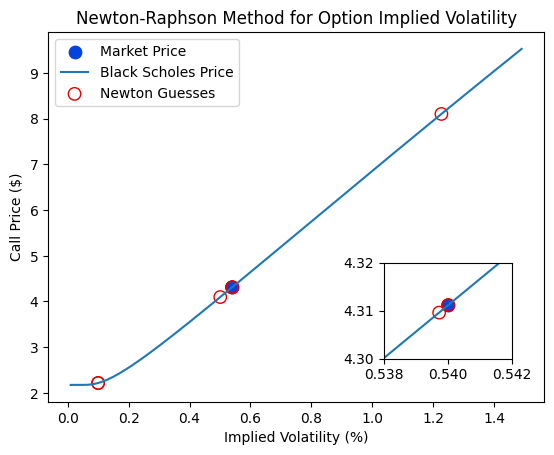
\includegraphics[width=0.85\linewidth]{images/call_newton}
\end{center}
\end{columns}
\end{frame}

\begin{frame}{Problems with the Black Model}
	\begin{itemize}
		\item It is widely used in practice as the metric by which traders translated volatilities into prices until rates became too low and the model collapsed under the assumption of positive rates.
		\item In the Black model \textcolor{red}{negative rates are not allowed}.
		\begin{equation*}
			d_{1,2} = \frac{\boxed{\log{\frac{F}{K}}} \pm \cfrac{v^2}{2}}{2} 
		\end{equation*}
		but in the last years in the inter-bank market it was not so unusual to find prices for -1\% strike floors.
		\item Moreover in the Black model the empirical evidence of the "smile" (volatility vs $K$) is not accounted for, i.e. $\sigma$ is a constant. Two caps identical but for the strike need a different volatility to recover two different market prices if one uses Black formula.
		%\item And this is clear if one looks at the distribution and at the process of $F(t, T, S)$; the volatility does not depend on the strike of the option. It is a characteristic of the forward rate.
	\end{itemize}
\end{frame}

\begin{frame}{The Practitioner Solutions}
	\begin{itemize}
		\item \textbf{"Smile" issue}: the model is used with \textcolor{red}{different input volatilities for different strikes}. In practice it is a mapping of implied volatilities into prices and vice versa.
		\item \textbf{Non-positive rates}: could have switched to a different dynamics, like ABM, where negative values are "normal". But there are large differences in the tails between normal and log-normal distributions.
		So Black model has been \textcolor{red}{shifted}. The technique was already known but in the last years has become crucial to shift the lower bound of prices admitted by the model.
	\end{itemize}
\end{frame}

\begin{frame}{Shifted Log-normal Model for Caplets}
	\begin{itemize}
		\item It can be shown that Black formula provides valid solutions if strike and forward rate are \textcolor{red}{shifted}. For a $(T,S)$ caplet with strike $K$ we get
		\begin{equation}
			\textbf{Cpl}_{Bl}(t,T,S,\tau,K,v_T,\alpha) = P(t,S) Bl(K+\alpha,F(t;T,S)+\alpha,v_T)
		\end{equation}
		where $d_1$ and $d_2$ read as before and instead $v_i$ is now given by
		\begin{equation*}
			v_i = \sigma^{\text{shifted}}\sqrt{T_{i-1}}
		\end{equation*}
		\item The market quotes of $\sigma^{\text{shifted}}$ refer to shifts $\alpha$ of the order of [2\%,3\%].
		%\item What is the relationship between $\sigma^{\text{shifted}}$ and $v_T$ ?
		%\item Rewrite the Black-76 SDE for the $(T, S)$ caplet as follows
		%\begin{equation}
		%	dF(t,T,S)=\sigma^{\text{shifted}}(F(t,T,S)-\alpha)dW^{\mathcal{Q}_S}(t)
		%\end{equation}
		%\item It is easy to see that the price for a $(T,S)$ caplet with strike $K$ is given by
		%\begin{equation}
		%	Cpl(t,T,S,\tau,K,v_T,\alpha)=P(t,S)Bl(K-\alpha,F(t,T,S)-\alpha,v_T)
		%\end{equation}
	\end{itemize}
\end{frame}

\begin{frame}[fragile]{Shifted Geometric Brownian Motion}
\begin{columns}
	\column{0.55\linewidth}
\begin{ipython}
import numpy as np

def GBM(mu, sigma, X0, T, steps, N):
    X = np.zeros(shape=(steps, N))
    dt = T/steps
    X[0, :] = X0
    eps = np.random.normal(size=(steps-1, N))
    X[1:, :] = np.exp((mu-0.5*sigma**2)*dt+sigma*np.sqrt(dt)*eps)
    return np.cumprod(X, axis=0)

def GBMShifted(mu, sigma, shift, X0, T, steps, N):
    X0_shifted = X0 + shift
    if (X0_shifted < 0.0):
        raise ValueError('Shift is too small !')

    X_shifted = GBM(mu, sigma, X0_shifted, T, steps, N)
    return X_shifted - shift
\end{ipython}
\column{0.4\linewidth}
\begin{ipython}
N = 10000
tsteps = 500
T = 3.0
sigma = 0.2
L0 = -0.05
shift = 0.1

paths = GBMShifted(0.0, sigma, shift, L0, T, tsteps, N)    
\end{ipython}
\begin{center}
	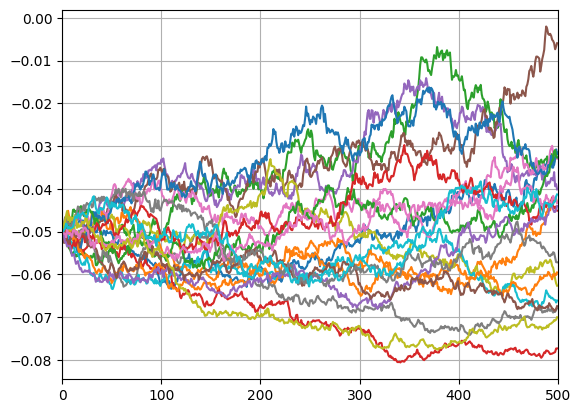
\includegraphics[width=0.9\linewidth]{images/shifted_gbm}
\end{center}
	\end{columns}
\end{frame}

\begin{frame}{Shifted Geometric Brownian Motion}
	\begin{center}
		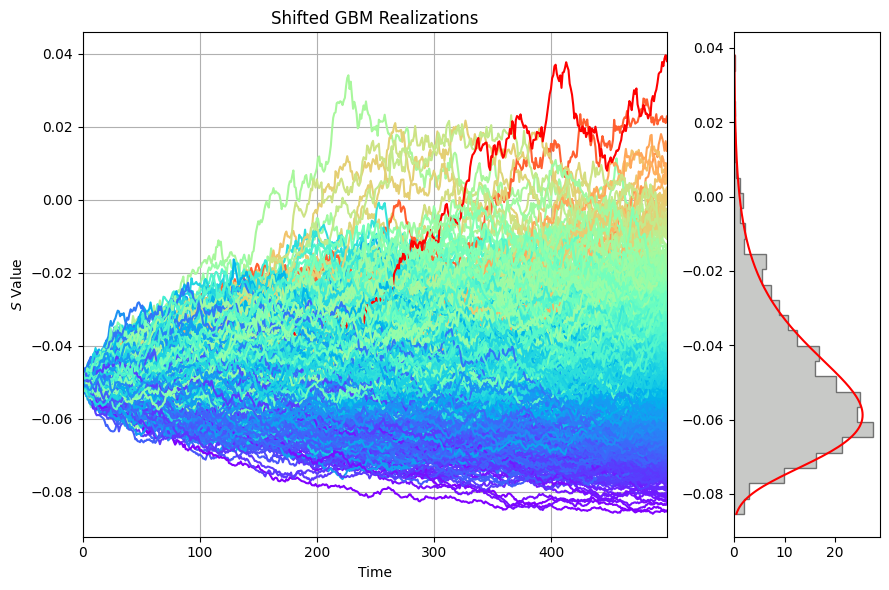
\includegraphics[width=0.7\linewidth]{images/shifted_gbm_density}
	\end{center}
\end{frame}

\begin{frame}{Shifted Log-normal}
	\begin{itemize}
		\item The density for the log-normal is:
		\begin{equation}
			\cfrac{1}{(x-\delta)\sigma\sqrt{2\pi}}e^{-\frac{1}{2\sigma^2}(\ln(x-\delta)-\mu)^2},\quad x>\delta, \mu\in\mathbb{R},\sigma >0
		\end{equation}
		\item In a \emph{Normal} distribution, $\mu$ plays the role of location-parameter, so "shifting" it is a trivial task.
		\begin{columns}
			\column{0.6\linewidth}
			\item In the log-normal instead $\mu$ is not a shift parameter, but a \emph{scale} parameter. It stretches and compresses rather than shifts ($\sigma$ is a shape parameter, controlling how skewed/heavy tailed the distribution is).
			\item Shifting the normal and then exponentiating to a log-normal is different from shifting the log-normal (the issue boils down to the fact that addition and exponentiation are not commutative).
			\column{0.4\linewidth}
			\begin{center}
				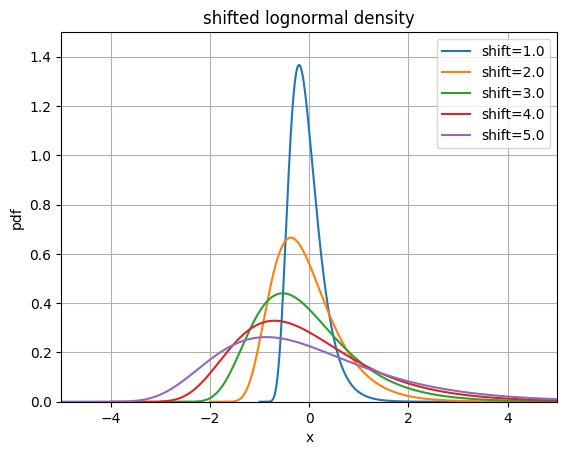
\includegraphics[width=0.95\linewidth]{images/shifted_lognormal}
			\end{center}
		\end{columns}
	\end{itemize}
\end{frame}

\begin{frame}[fragile]{Shifted Black Formula}
	Compare the result for Cap Black formula to the Monte Carlo simulation both with a shift $\Delta$.
	\begin{columns}
		\column{0.5\linewidth}
		\begin{ipython}
import numpy as np
			
def BS_shifted(St, K, shift, r, sigma, ttm):
    K_shifted = K + shift
    St_shifted = St + shift
    return BS(St_shifted, K_shifted, r, sigma, ttm)
			
T = 3.0
sigma = 0.2
L0 = -0.05
shift = 0.1
r = 0
			
K = np.linspace(-shift, np.abs(L0)*3, 25)
optPriceMCV = np.zeros([len(K), 1])
for idx in range(len(K)):
    optPriceMCV[idx] = np.mean(np.maximum(paths[-1, :] - \
                               K[idx], 0.0))
			
optPriceExact = BS_shifted(L0, K, shift, r, sigma, T)
\end{ipython}
\column{0.5\linewidth}
\begin{center}
	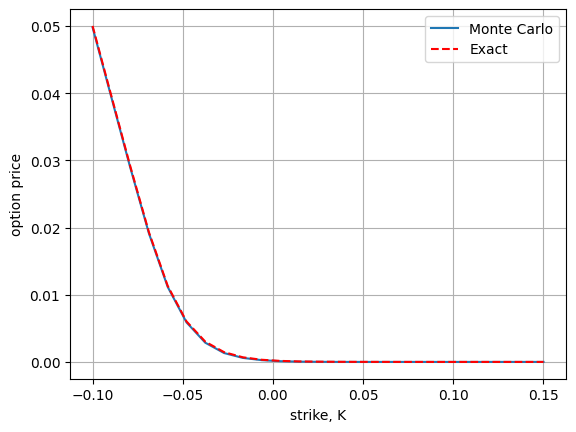
\includegraphics[width=0.65\linewidth]{images/shifted_call_BS_vs_MC}\\
	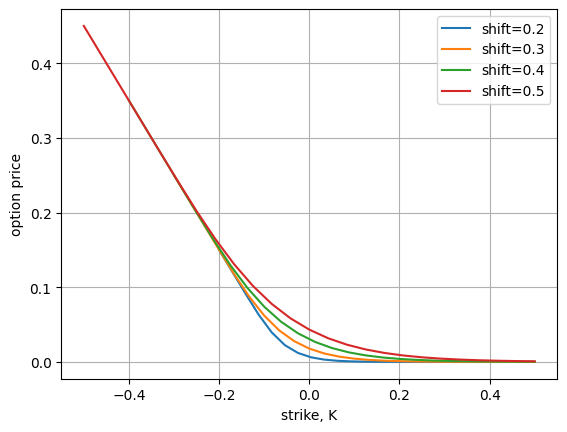
\includegraphics[width=0.65\linewidth]{images/shifted_call}
\end{center}
\end{columns}
\end{frame}


%\begin{frame}{The Volatility Hump}
%\begin{itemize}
%	\item Empirical studies have pointed out two very important facts:
%	\begin{itemize}
	%		\item the first one is that interest rates volatility can depend on the level of the interest rates themselves;
	%		\item moreover the volatility function is increasing in the short end of the curve, and decreasing in the long end, with an \textcolor{red}{humped} type movement.
	%	\end{itemize}  
%	\begin{columns}
	%		\column{0.45\linewidth}
	%		\item Uncertainty is bigger in the intermediate region and lower in the front of the maturity spectrum. For long maturities volatility tends to decay.
	%		\item When the hump does not appear it is regarded as \emph{stressed market}.
	%		%\item There is a financial explanation for this feature.
	%		\column{0.45\linewidth}
	%		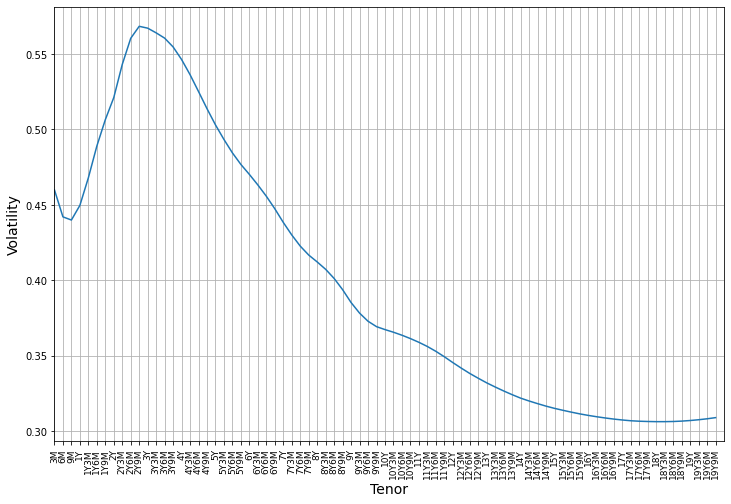
\includegraphics[width=1.1\linewidth]{cap_vola}
	%	\end{columns}
%\end{itemize}
%\end{frame}

%\begin{frame}{Swaptions Volatility Calibration}
%\begin{itemize}
%	\item Swaption volatilities are quoted for different maturities and tenors (length of the underlying swap).
%	\item Both for ATM and away from ATM on both sides ("swaption smile").
%	\item So swaptions have an additional dimension with respect to caps: the quotes are parametrized according to 
%	\begin{itemize}
%		\item maturites;
%		\item tenors;
%		\item strikes.
%	\end{itemize}
%	%\item They have also a different \emph{delta} effect on your book.
%	%		\item Volatility trade between caps ans swaption: WEDGE
%\end{itemize}
%\end{frame}
%
%\begin{frame}{Swaption Volatility Calibration}
%  \begin{center}
%    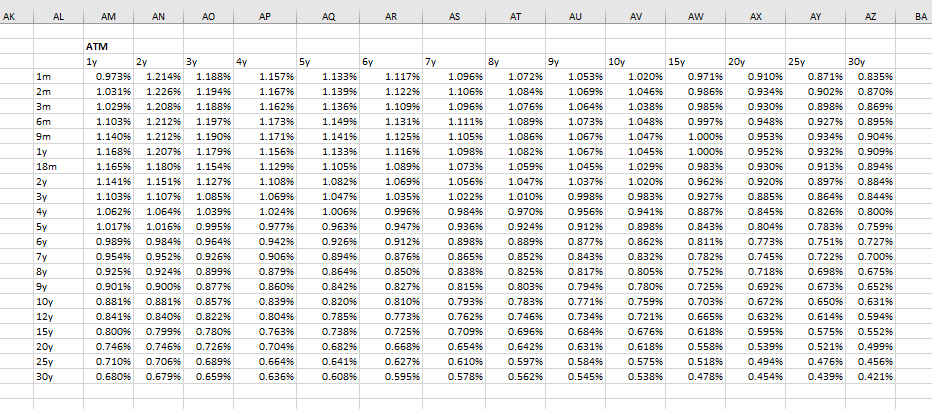
\includegraphics[width=1.\linewidth]{images/atm_vol}
%  \end{center}
%\end{frame}
%
%\begin{frame}{Swaption Volatility Calibration}
%  \begin{center}
%    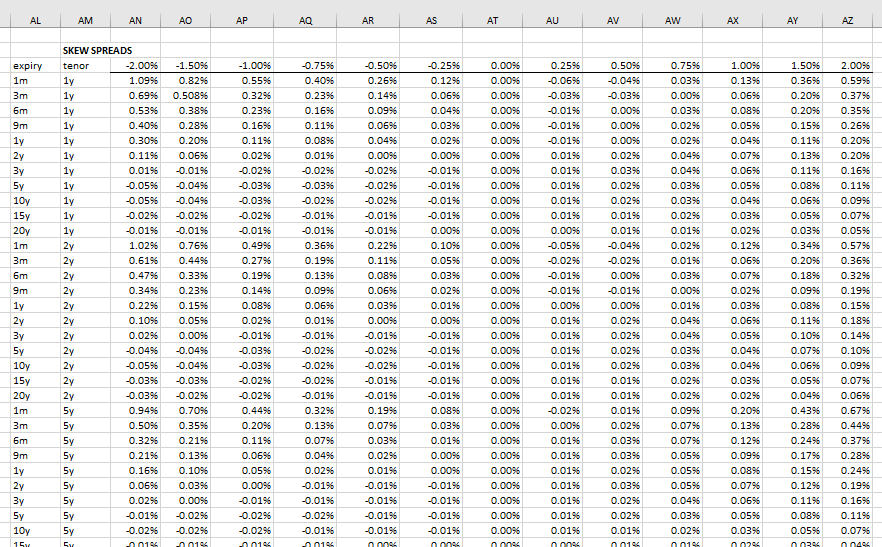
\includegraphics[width=1.\linewidth]{images/skews}
%  \end{center}
%\end{frame}
%
%\begin{frame}{Swaption Volatility Calibration}
%  After we have constructed the volatility matrix we can fit the ``smile'' at each (expiry, tenor) pair.
%
%  This is done assuming the volatilities evolves according to the SABR model. An approximated solution has been given by \emph{Hagan et al.}
%  \begin{eqnarray} \sigma _{B}(K,f) &=&\frac{\textcolor{red}{\alpha} \left\{ 1+\left[ \frac{\left( 1-\textcolor{red}{\beta} \right) ^{2}}{24}\frac{\textcolor{red}{\alpha} ^{2}}{(fK)^{1-\textcolor{red}{\beta}}}+\frac{1}{4}\frac{\textcolor{red}{\rho \beta \nu\alpha}}{(fK)^{(1-\textcolor{red}{\beta})/2}}+\frac{2-3\textcolor{red}{\rho} ^{2}}{24}\textcolor{red}{\nu}^{2}\right] T\right\} }{(fK)^{(1-\textcolor{red}{\beta})/2}\left[ 1+\frac{(1-\textcolor{red}{\beta})^{2}}{24}\ln ^{2} \frac{f}{K}+\frac{(1-\textcolor{red}{\beta})^{4}}{1920}\ln^{4}\frac{f}{K}\right] } \times \frac{z}{\chi (z)} \notag \\ z &=&\frac{\textcolor{red}{\nu}}{\textcolor{red}{\alpha}}(fK)^{(1-\textcolor{red}{\beta})/2}\ln \frac{f}{K} \notag \\ \chi (z) &=&\ln \left[ \frac{\sqrt{1-2\rho z+z^{2}}+z-\textcolor{red}{\rho}}{1-\textcolor{red}{\rho}}\right] . \notag \end{eqnarray}
%\end{frame}
%
%\begin{frame}{Swaption Volatility Calibration}
%    \begin{center}
%      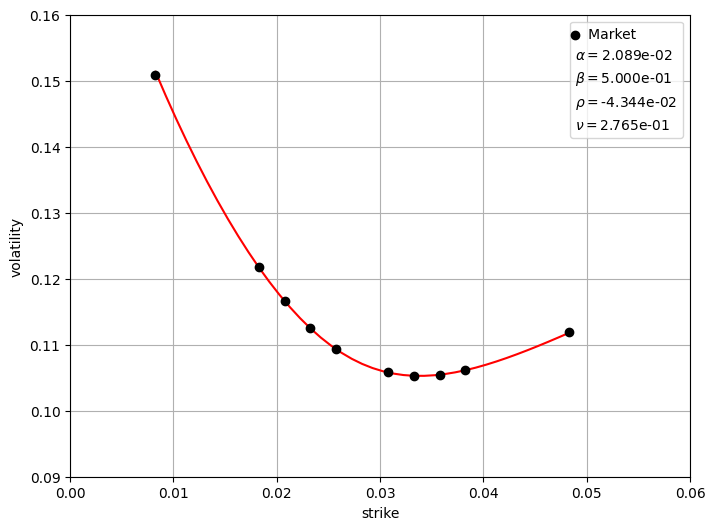
\includegraphics[width=0.65\linewidth]{images/10y_10y}
%    \end{center}
%\end{frame}
%
%\begin{frame}{Swaption Volatility Calibration}
%    \begin{center}
%      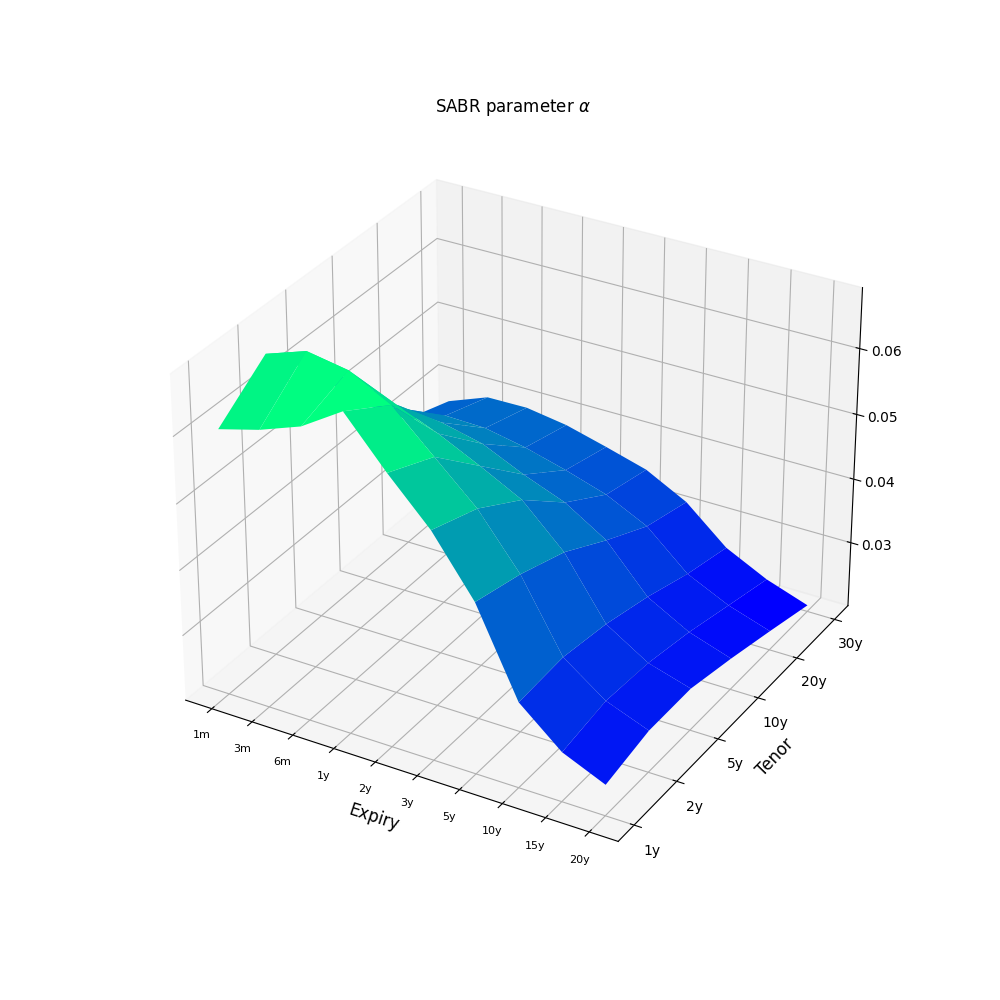
\includegraphics[width=0.3\linewidth]{images/alpha}
%      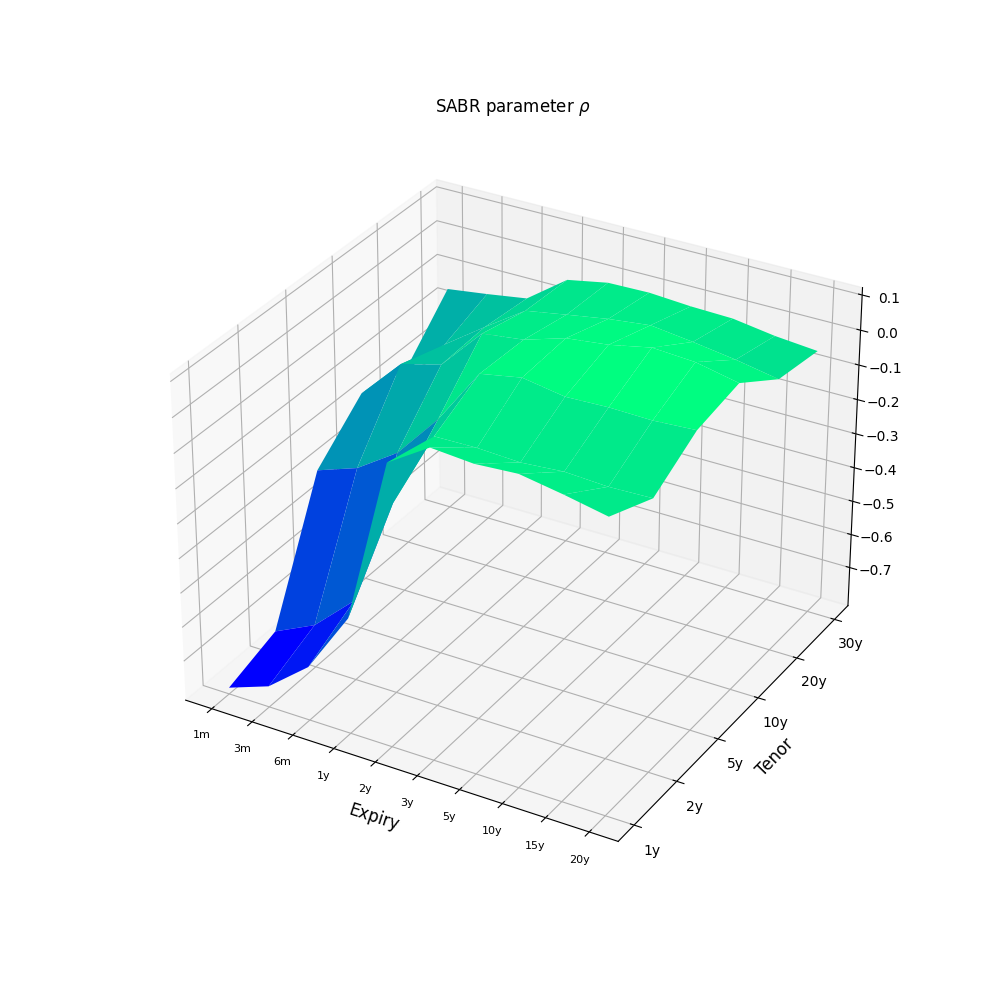
\includegraphics[width=0.3\linewidth]{images/rho}
%      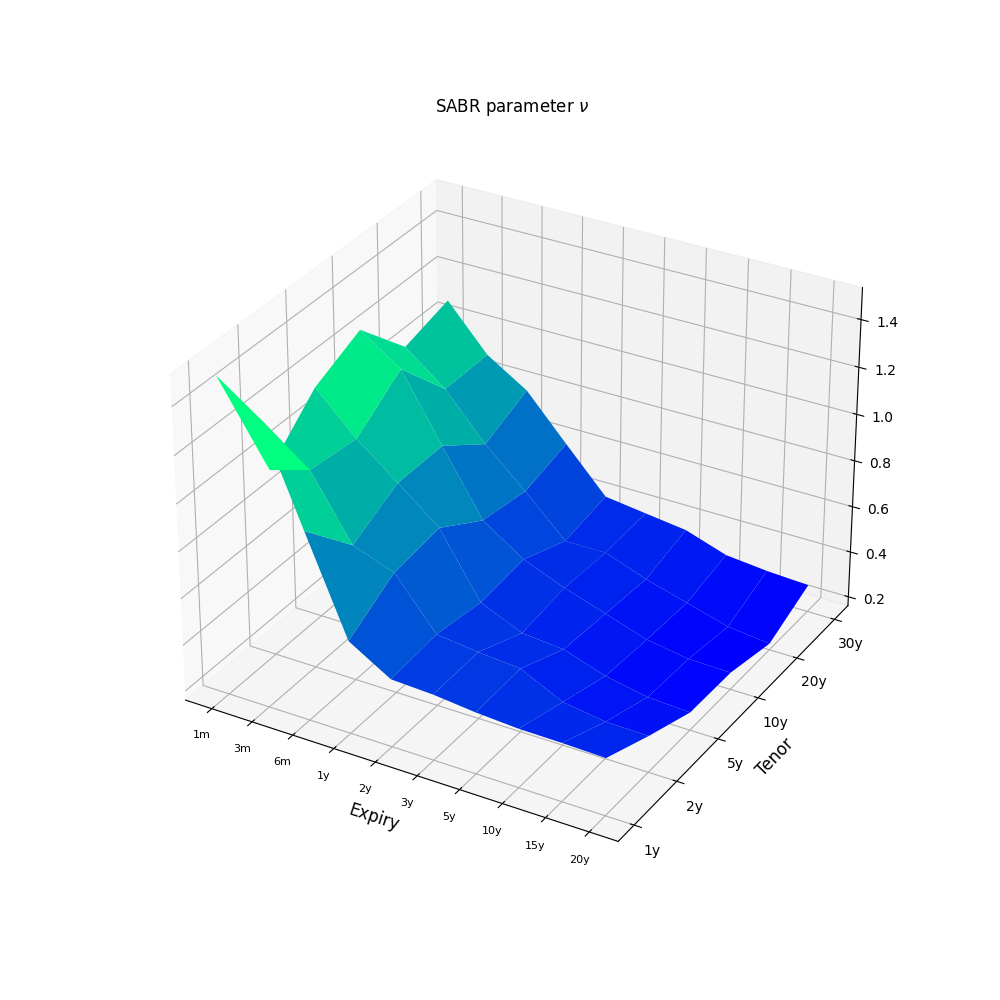
\includegraphics[width=0.3\linewidth]{images/nu}
%    \end{center}
%\end{frame}


%\begin{frame}{Differences between Caps and Swaptions}
%\begin{itemize}
%	\item<1-> Caps can be decomposed into more elementary products: \textcolor{red}{caplets}. Value each caplet one by one and then add their prices
%	\begin{itemize}
%		\item each forward rate can be modeled as a random variable;
%		\item \textbf{no joint action of forward LIBOR rates is involved.}
%	\end{itemize}
%	\item<2-> Unfortunately this is not possible with swaptions. The swap rate is \textcolor{red}{essentially a weighted average of forward rates} $S=\frac{\sum F(t;T_{i-1},T_i)}{\sum P(t,T_i)}$, hence its volatility should depend on each forward rate volatilities \textbf{as well as} their correlations.
%	\item<3-> If you take as "fundamental" entity the LIBOR rates you have to deal with the joint action of the simple forward LIBOR rates and so with the \textbf{terminal correlation} between rates of different portions of the yield curve. 
%	\item<4-> This issue will be extensively studied in the context of the Libor Market Models further on down the course.
%	%Can you provide an example ?
%\end{itemize}
%\end{frame}

\section{Bond Options}
\begin{frame}{An Option to Exchange Fixed with Float}
\begin{itemize}
	\item<1-> We have seen that a Swap can be viewed as an exchange of bonds (fixed for float).
	\item<1-> Hence a Swaption can be regarded as an \textcolor{red}{option to exchange fixed for floating} bonds (or vice versa).
	\item<2-> In case it would be possible to get a simple expression for a \textcolor{red}{Coupon Bond Option} we could use to price Swaptions.
	\item <2-> It would be even simpler if we could express a Coupon Bond Option as a portfolio of Zero Coupon Bond Options.
	\item<3-> Luckily we can do that thanks to a recipe known as \textcolor{red}{Jamshidian's decomposition}.
\end{itemize}
\end{frame}

\begin{frame}{Jamshidian's Decomposition}
\begin{block}{Theorem}
	Consider a sequence of functions $f_i$, a random variable $W$ and a constant $K\ge0$. If each $f_i$ is monotone (decreasing), that is $\cfrac{\partial f_i}{\partial W} < 0;\;\forall i$, then 
	\begin{equation*}
		\left(K - \sum_i f_i(W)\right)^+ = 	\sum_i \left(K_i - f_i(W)\right)^+
	\end{equation*} 
	In financial terms it means that the payoff of an option on a portfolio of assets can be expressed in terms of a portfolio of options on each asset.
\end{block}
\end{frame}

\begin{frame}{Jamshidian's Decomposition Proof}
\begin{itemize}
	\item<1-> Since each $f_i$ is monotone also $\sum_i f_i$ is decreasing. Hence there is a unique solution $\hat{w}$ to 
	\begin{equation*}
		\sum_i f_i(\hat{w}) = K   
	\end{equation*}
	\item<2-> Each $f_i$ is decreasing so
	\begin{columns}
	\column{0.7\linewidth}
	\uncover<2->{\begin{equation*}
	\left(K - \sum_i f_i(W)\right)^+ = \left(\sum_i f_i(\hat{w}) -  \sum_i f_i(W)\right)^+ = 
	\end{equation*}}
	\uncover<3->{\begin{equation*}
	= \left(\sum_i (f_i(\hat{w}) -  f_i(W))\right)^+= \sum_i (f_i(\hat{w}) - f_i(W))\mathbbm{1}_{W\ge \hat{w}}
	\end{equation*}}
	\uncover<4->{\begin{equation*}
	= \sum_i \left(K_i - f_i(W)\right)^+\quad\qedsymbol
	\end{equation*}
	}
	\column{0.35\linewidth}
	\uncover<1->{
	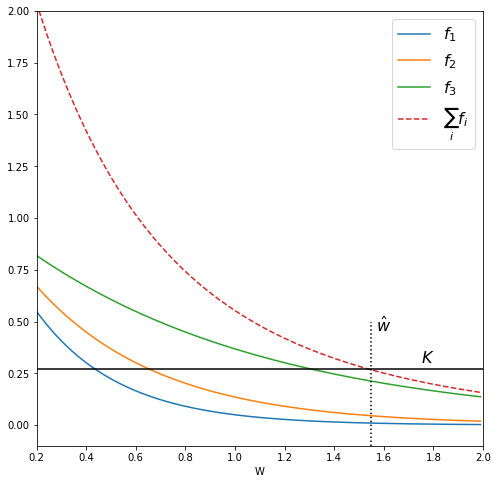
\includegraphics[width=1\linewidth]{images/jamshidian_trick}}
\end{columns}
\end{itemize}
\end{frame}

\begin{frame}[fragile]{Jamshidian Decomposition Example}
\begin{columns}
    \column{0.5\linewidth}
    \begin{ipython}
import numpy as np

def psi(t_i, X):
  return np.exp(-t_i*np.abs(X))

def sumPsi(N, X, psi):
  A = 0
  for t_i in range(0, N):
    A += psi(t_i, X)
  return A

nsimulations = 1000; N = 15
X = np.random.normal(size=nsimulations)
K = np.linspace(2, 10, 100)
resultMC = np.zeros(len(K))
sum_of_functions = sumPsi(N, X, psi)
for i, Ki in enumerate(K):
  resultMC[i] = np.mean(np.maximum(sum_of_functions - Ki, 0))
    \end{ipython}
    \column{0.5\linewidth}
Consider the process
\begin{equation*}
\psi_i(X)=e^{-t_i}|X|,\quad t_i=\{0,1,2,\ldots, N\}
\end{equation*}
with $X\approx\mathcal{N}(0,1)$ and compute
\begin{equation*}
A = \mathbb{E}\left[\max\left(\sum_{k=1}^N \psi_k(X) - K, 0\right)\right]  
\end{equation*}    
\end{columns}
\end{frame}

\begin{frame}[fragile]{Jamshidian Decomposition Example}
\begin{columns}
    \column{0.5\linewidth}
    \begin{ipython}
import numpy as np
from scipy.optimize import newton

def objective(x, psi, N, K):
    temp = 0
    for i in range(0, N):
        temp += psi(i, x)
    return temp - K

def jamshidian_decomposition(psi, N, K):
    result = newton(objective, 0.1, args=(psi, N, K))
    return result

nsimulations = 1000; N = 15
X = np.random.normal(size=nsimulations)
K = np.linspace(2, 10, 100)
resultJams = np.zeros(len(K))
for i, Ki in enumerate(K):
  optK = jamshidian_decomposition(psi, N, Ki)
  A = 0
  for j in range(0, N):
    A += np.mean(np.maximum(psi(j, X) - psi(j, optK), 0))
  resultJams[i] = A
    \end{ipython}
    \column{0.5\linewidth}
The $\psi_i$ are monotonic decreasing so we can apply Jamshidian decomposition
\begin{equation*}
A = \mathbb{E}\left[\sum_{i=1}^N \max(\psi_i(X) - \psi_i(X^*), 0)\right]
\end{equation*}
with $\sum_{i=1}^N \psi_i(X^*) = K$
\end{columns}
\end{frame}

\begin{frame}{Jamshidian Decomposition Example}
\begin{center}
    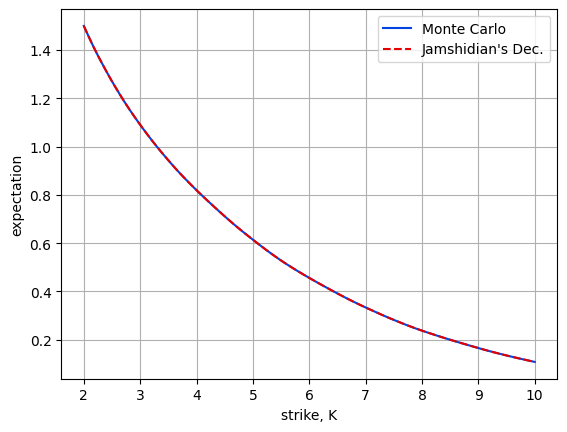
\includegraphics[width=0.65\linewidth]{images/jamshidian_ex1}
\end{center}
\end{frame}

\begin{frame}{Back to Coupon Bond Option}
\begin{itemize}
	\item<1-> Consider a coupon bond which pays the following cash flows $\mathcal{C}=\{c_1,\dots,c_n\}$ at dates $\mathcal{T}=\{T_1,\ldots,T_n\}$.
	\item<2-> Let $t\leq T_1$, the bond price is given by
	\begin{equation*}
		\textbf{CB}(t,\mathcal{C},\mathcal{T})=\sum_{i=1}^n c_i \Pi(t, T_i, r(t))
	\end{equation*}
	\item<3-> Suppose we would like to calculate the price of a put option with strike $K$ on this coupon bond. The payoff reads
	\begin{equation*}
		\textbf{CBP}=\left[K-\textbf{CB}(t,\mathcal{C},\mathcal{T})\right]^+ = \left[K-\sum_{i=1}^n c_i \Pi(t, T_i, r(t))\right]^+
	\end{equation*}
\end{itemize}
\end{frame}

\begin{frame}{Coupon Bond Option}
\begin{itemize}
	\item<1-> Now apply the Jamshidian's decomposition to previous payoff.
	\item<2-> First need to find the interest rate value $r^*$ such that $\sum_{i=1}^n c_i \Pi(t, T_i, r^*) = K$.
	\item<3-> Assuming the interest rate model satisfies the required condition (which is true for Short Rate models for example)
	\begin{equation*}
		\frac{\partial \Pi(t,T_i,r(t))}{\partial r}<0,\;\forall 0<t<s
	\end{equation*}
	we can write the payoff as
	\begin{equation}
		\textbf{CBP}(t,T_i,\Pi,r^*) = \sum_{i=1}^n c_i [\Pi(t, T_i, r^*)-\Pi(t, T_i, r(t))]^+
	\label{eq:bond_option_payoff}
	\end{equation}
\end{itemize}
\end{frame}

\begin{frame}{Coupon Bond Option}
\begin{itemize}
	\item \cref{eq:bond_option_payoff} tells us that we can price a coupon bond option as a portfolio of options on ZCBs.
	\item The strike of these option is calculated as the value of a ZCB given a \emph{particular} value of the short rate, determined with a root finding procedure.
	\item In formulas the CBO with maturity $T$ and strike $K$ reads
	\begin{equation}
		\boxed{\textbf{CBP}(t,\mathcal{T},\mathcal{C},K) = \sum_{i=1}^n c_i \textbf{ZBP}(t,T_i,\Pi,r^*)}
	\end{equation}
\end{itemize}
\end{frame}

\begin{frame}{Swaption Pricing under Affine Models}
\begin{itemize}
	\item When interest rates are modeled using \textcolor{red}{Affine Short Rate Models} (Vasicek, Hull-White,\ldots) swpation pricing can be performed semi-analytically.
	\item \cref{eq:swaption_payoff_std} can be rewritten, expressing the underlying swap in terms of bonds, as
\begin{equation*}
\textbf{PSw}=NP(t_0, T_\alpha)\mathbb{E}_t\left[\max\left(1-\sum_{k=\alpha+1}^\beta c_kP(T_\alpha,T_k), 0\right)\right]
\end{equation*}
with $c_k=K\tau_k$ for $k=\alpha+1,\ldots,\beta-1$ and $c_\beta=(1+K\tau_\beta)$.
	\item One of the most striking properties of \emph{Affine Models} is that they relate ZCB price to a spot rate modeled according to 
	\begin{equation*}
		P(t,T) = A_r(t,T)e^{-B_r(t,T)r}
	\end{equation*} 
\end{itemize}
\end{frame}

\begin{frame}{Swaption Pricing under Affine Models}
\begin{itemize}
\item Hence
\begin{equation*}
\textbf{PSw}=NP(t_0, T_\alpha)\mathbb{E}_t\left[\max\left(1-\sum_{k=\alpha+1}^\beta c_k A_r(\tau_k)e^{B_r(\tau_k)r(T_\alpha)}, 0\right)\right]
\end{equation*}
	\item Using the Jamshidian decomposition the $\max$ operator can be swapped with the sum
\begin{equation*}
\textbf{PSw}=NP(t_0, T_\alpha)\sum_{k=\alpha+1}^\beta c_k \mathbb{E}_t\left[\max\left(\bar{K_k} - A_r(\tau_k)e^{B_r(\tau_k)r(T_\alpha)}, 0\right)\right]
\end{equation*}
whit $\bar{K_k} := A_r(\tau_k)e^{B_r(\tau_k)r^{*}}$, where the parameter $r^{*}$ is determined by solving
\begin{equation*}
\sum_{k=\alpha+1}^\beta c_k \left(A_r(\tau_k)e^{B_r(\tau_k)r^{*}}\right) = 1
\end{equation*}
\end{itemize}
\end{frame}

\begin{frame}{Swaption Pricing under Affine Models}
\begin{itemize}
\item As noted above for the bond options, each element of the sum in the formula above represents a European put option on a zero-coupon bond, which in the \emph{affine models} has a closed-form solution.
\item So a payer swaption price is thus given by
	\begin{equation}
		\boxed{\textbf{PSw}(t,T,N) = N\sum_{k=1}^n c_k \textbf{ZBP}(t,T_k,K_k)}
	\end{equation}
	while the receiver swaption price reads
	\begin{equation}
		\boxed{\textbf{RSw}(t,T,N) = N\sum_{k=1}^n c_k \textbf{ZBC}(t,T_k,K_k)}
	\end{equation}
\end{itemize}	
\end{frame}

\begin{frame}[fragile]{Swaption Pricing with Vasicek Model}
Implement the Jamshidian decomposition to price swaptions under the Vasicek short rate model $dr = k(\theta - r_t)dt + \sigma dW$.
\begin{columns}
\column{0.5\linewidth}
\begin{ipython}
from scipy.optimize import newton

def obj(r, model, K, tenor, terms):
  val = 0
  for i, T in enumerate(terms):
    val += model.ZCB(r, T-1, T)*K*tenor
  val += model.ZCB(r, T-1, T)
  return val-1

def rstar(terms, model, tenor, K):
  return newton(obj, 0.01, args=(model, K, tenor, terms))

def npv(model, notional, K, terms, tenor, r, r_star, option_type):
  val = 0
  for i, T in enumerate(terms):
    K_k = model.ZCB(r_star, T-1, T)
    val += model.ZBO(r, K_k, 0, T-1, T, option_type)*K*tenor
  val += model.ZBO(r, K_k, 0, T-1, T, option_type)
  return notional*val
\end{ipython}
\column{0.5\linewidth}
\vspace{2.5cm}
\begin{ipython}
expiry = 1; tenor=2
vasicek = Vasicek(theta=0.005, kappa=0.03, sigma=0.04)
terms = np.linspace(expiry+1, expiry+tenor, tenor)
r_star = rstar(terms, vasicek, tenor=2, K=0.02)
print (f"r_star: {r_star:.4f}")
# Notice that we are dealing with a 
# Payer Swaption so the option type has to be Put
npv = npv(vasicek, notional=1e6, K=0.02, terms, 
          tenor, r=0.03, r_star, OptionType.Put)
print (f"Swaption NPV: {npv:,.2f}")
\end{ipython}
\begin{ioutput}

r_star: 0.0783
Swaption NPV: 4,374.78
\end{ioutput}
\end{columns}
\end{frame}

\subsection{Bermudan Swaption}
\begin{frame}{Bermudan Swaptions}
\begin{itemize}
	\item<1-> It is a swaption in which the optionality can be exercised at a \textcolor{red}{predetermined set of dates} (not only one).
	\item<2-> It is useful for hedging callable bonds (especially if step-up, i.e. with the coupon increasing with time).
	\item<3-> A \textcolor{red}{Bermudan Swaption} gives the holder the right but not the obligation to enter in an interest rate swap contract at different dates (usually the swap reset dates) with some days of notification to the counter-party.
	\item<4-> The interest rate swap the holder can enter into, is the same existing contract, so if the holder does not exercise at the first date in the call schedule, the option for the following periods is just written on shorter swaps.
\end{itemize}
\end{frame}

\begin{frame}{Bermudan Swaption Example}
\begin{itemize}
	\item<1-> As an example consider the following: receiver Bermudan Swaption written on a 3 years swap with the first call date $2y$ from now (we suppose semi-annual payments).
	\item<2-> If at the end of the second year she will not exercise, six months later she will have to decide if entering or not in the same remaining swap which now has become a $2y6m$ swap.
	\item<3-> If again she will not exercise the last possibility will involve the decision of whether or not to enter on the $2y6m-3y$~$FRA$.
\end{itemize}
\end{frame}		

%\begin{frame}{Bermudan Swaption Payoff}
%\begin{itemize}
%	\item At the maturity $T$, the payoff of a Bermudan swaption is given by
%	\begin{equation*}
%%		\textbf{BS}(T) = \max(0, V_{\text{swap}}(T))
%%	\end{equation*}
%%	where $V_{swap}(T)$ is the value of the underlying swap in $T$.
%%	\item At any exercise date $T_i$, the payoff of the Bermudan swaption is given by
%%	\begin{equation*}
%%	\textbf{BS}(T_i) = \max(K(T_i), V_{\text{swap}}(T_i))
%%	\end{equation*}
%%	where $V_{\text{swap}}(T_i)$ is the exercise value of the swap and $K(T_i)$ is the intrinsic value, i.e. the holder of the option receives $\max(K(T_i), 0)$ if the option is exercised at time $T_i$.
%%	CONTROLLARE ULTIMO DISCORSO
%%\end{itemize}
%%\end{frame}

\begin{frame}{Bermudan Swaption Pricing}
\begin{itemize}
	\item<1-> Some interest rate instruments can be priced just looking at the term structure of interest rates (FRA and Swaps)
	\begin{itemize}
		\item the only problem is: which is the right term structure ? (this is a lesson from the 2008 crisis).
	\end{itemize}
	\item<2-> Some other instruments cannot be priced only with the yield curve: we need the future (risk-neutral) evolution of the rates.
	%\item Non-linearities come in !
	%\item Swaptions are non-linear products and may require to model the correlation between forward LIBOR rates.
	\item<3-> Given the complexity of Bermudan swaption valuation (which belongs to the latter class), there is no closed form solution.		
	\item<4-> Typically tree techniques or the Longstaff-Schwartz method are used.
\end{itemize}
\end{frame}

\begin{frame}{Longstaff-Schwartz Algorithm}
\begin{itemize}
    \item Consider a Bermudan put option with strike $K$ and $n$-years maturity. Each year you can choose whether to exercise or not.
    %Let's implement a MC which actually simulates, besides the evolution of the market, what an investor holding this option would do.
    \item The evolution of the asset value and of the money market account gives
    \begin{equation}
	\begin{gathered}
		S(t_1=1y) = S(t_0)e^{(r-\frac{1}{2}\sigma^2)(t_1-t_0)+\sigma\sqrt{t_1-t_0}\mathcal{N}(0,1)} \\
		B(t_1=1y)=B(t_0)e^{r(t_1-t_0)}
	\end{gathered}
    \end{equation}
    \item \emph{At this point how does the investor know if it is convenient to exercise?}
    \begin{itemize}
        \item \textbf{Exercise:} in this case we knows exactly the payoff;
        \item \textbf{No Exercise:} the contract has become a European Put Option with shorter maturity.
    \end{itemize}
    \item The decision will depend on each choice convenience:
    \begin{equation*}
\max[K-S(t_1), P(t_1,T;S(t_1),K)]
    \end{equation*}
where $P(t_1,T;S(t_1),K)$ is the price of a Put which can be computed analytically (i.e. the \emph{continuation value}, the value of holding the option instead of early exercising it).
\end{itemize}
\end{frame}

\begin{frame}{Longstaff-Schwartz Algorithm}
\begin{itemize}
    \item So the premium of the option is the average of this discounted payoffs calculated in each Monte Carlo simulation
\begin{equation*}
	\cfrac{1}{N}\sum_i\max[K-S(t_1), P(t_1,T;S(t_1),K)]
\end{equation*}
    \item In this case we could price this product because we have an analytical pricing formula for the Put, but what if we didn't ?
    \item \textbf{Brute force solution:} for each realization of $S(t_i)$ we run another Monte Carlo to price the alternative continuation value.
    \item We need to implement nested MC which is usually a very bad idea. Its execution time grows as $N^2$, which becomes prohibitive when you deal with multiple exercise dates !
\end{itemize}    
\end{frame}

\begin{frame}{Longstaff-Schwartz Algorithm}
Let's search for a smarter solution analyzing the relationship between the continuation value and the realizations of $S$ at step $t_1$.
%We can plot the discounted payoff at maturity, $P_i$ vs $S_i(t_1)$.
\begin{columns}
\column{0.5\linewidth}
    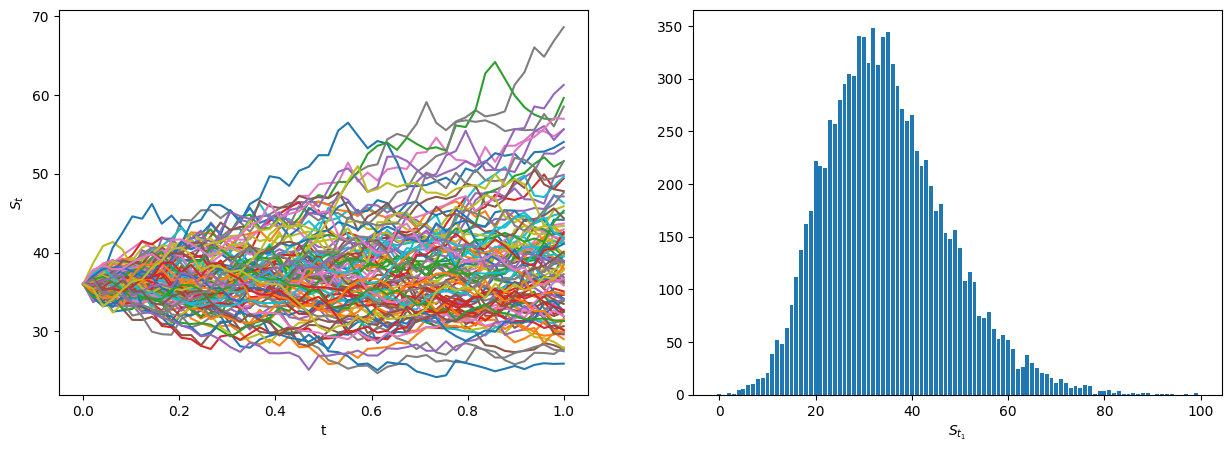
\includegraphics[width=0.9\linewidth]{images/longstaff_simulation}
    
    \small{The analytical price of the put (green line) interpolates the cloud of MC points, so \emph{the price at time $t_1$ can be computed by means of an average on all discounted payoff} (i.e. the barycentre of the cloud made of discounted payoff).}
\column{0.5\linewidth}    
    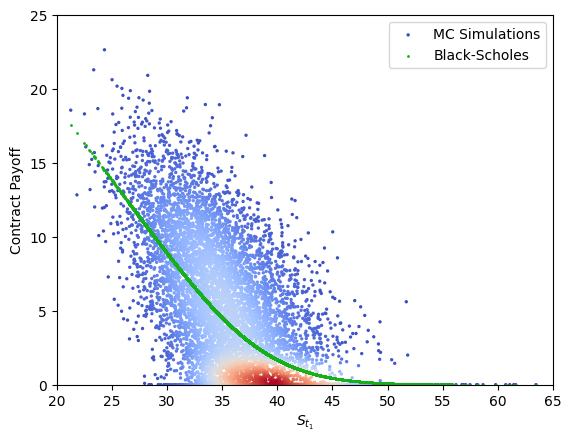
\includegraphics[width=0.9\linewidth]{images/longstaff_scatter_1}
\end{columns}

\textbf{Estimating the future value of an option can be seen as the problem of finding the curve that best fit the cloud of discounted payoffs at the date of interest.}
\end{frame}

\begin{frame}{Longstaff-Schwartz Algorithm}
\begin{center}
    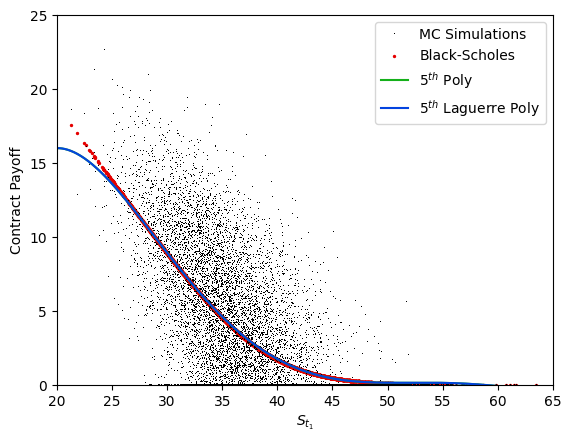
\includegraphics[width=0.35\linewidth]{images/longstaff_scatter_2}
\end{center}

\begin{itemize}
    \item So we have found an \emph{empirical pricing formula} for the unknown contract to be used in the Monte Carlo Simulation
\begin{equation}
	P(t_i,T,S(t_i),K)=c_0+c_1 S(t_i) + c_2 S(t_i)^2 + c_3 S(t_i)^3 + c_4 S(t_i)^4 + c_5 S(t_i)^5
\end{equation}
    The formula is obviously fast, the cost of the algorithm being just the best fit. 
    \item Clearly we could have used any form for the curve (not only a polynomial), but small improvement does not justify the increased complexity.
\end{itemize}
\end{frame}

\begin{frame}[fragile]{American Option Pricing}
\begin{columns}
\column{0.5\linewidth}
\begin{ipython}
import numpy as np

def longstaff_schwartz(S0, r, sigma, K, 
                       tsteps, T, N, side=OptionType.Call):
    dt = T / tsteps
    df = np.exp(-r*dt)
    S = GBM(r, sigma, S0, T, tsteps, N)

    h = np.maximum(side*(S-K), 0)

    V = h[-1]
    for t in range(tsteps-1, 0, -1):
        regr = np.polyfit(S[t], V*df, 5)
        C = np.polyval(regr, S[t])
        V = np.where(h[t]>C, h[t], V*df)
    return df*np.mean(V)    
\end{ipython}
\column{0.5\linewidth}
\vspace{2.5cm}
\begin{ipython}
S0 = 36.
K = 40.
T = 1.0
r = 0.06
sigma = 0.2

I = 25000
M = 50

V0 = longstaff_schwartz(S0, r, sigma, 
                        K, M, T, I, side=OptionType.Put)
print (f"American put option value {V0:5.3f}")    
\end{ipython}
\begin{ioutput}

American put option value 4.415
\end{ioutput}
\end{columns}
\end{frame}


%%\begin{frame}{Bermudan Swaption Pricing: Outline}
%%	\begin{itemize}
%%	\item<1-> Consider a tenor structure $\mathcal{T}=\{T_i\}^\beta_{i=\alpha}$ and a Bermudan receiver swaption with time $t$ value $\textbf{RBS}(t,K)$.
%%	\item<2-> Assuming no prior exercise, at any time point $T_i$ the swaption holder has the right to receive the exercise value $V_e$ of the swaption, i.e., present value of the underlying swap:
%%	\begin{equation}
%%	V_e(T_i)=(K-S_{i,\beta}(T_i))+\sum^\beta_{k=i+1} P(T_i,T_k)\tau_k
%%	\label{eq:exercise_value}
%%	\end{equation}
%%	\item<3-> The exercise value has to be compared to the so-called continuation value, $V_c$, of holding the option beyond $T_i$:
%%	\begin{equation}
%%	V_c(T_i)=\mathbb{E}[\textbf{RBS}(T_{i+1},K)|S_{i,\beta}(T_i)]
%%	\label{eq:continuation_value}
%%	\end{equation}
%%\end{itemize}
%%\end{frame}
%%
%%\begin{frame}{Bermudan Swaption Pricing: Outline}
%%	\begin{itemize}
%%		\item<1-> The value of the Bermudan swaption can now be given in terms of \cref{eq:exercise_value} and \cref{eq:continuation_value}, recursively.
%%		\item<2-> The evaluation of proceeds backward in time: at $T_{\beta-1}$
%%		the value of the Bermudan is known, i.e. the swaption payoff
%%		\begin{equation*}
%%			\textbf{RBS}(T_{\beta-1},K)=P(T_{\beta-1},T_\beta)\tau_\beta(K-S_{\beta-1,\beta}(T_{\beta-1}))^+
%%		\end{equation*}
%%		\item <3->This allows to update the continuation value at $T_{\beta-2}$ with \cref{eq:continuation_value} and compare it to the exercise value
%%		\begin{equation*}
%%			\textbf{RBS}(T_j,K)=\max(V_e(T_j),V_c(T_j)),\quad\text{for }j=\beta-2,\beta-3,\ldots,n
%%		\end{equation*}
%%	\end{itemize}
%%\end{frame}
%%
%%\begin{frame}{Bermudan Swaption Pricing: Outline}
%%	\begin{itemize}
%%		\item<1-> This procedure of comparing “backwardly-cumulated” continuation value with exercise value and deciding upon a swaption exercise is repeated until the initial valuation date is reached, at which point the algorithm yields a price estimate for the Bermudan swaption. 
%%		\item<2-> The calculation of the continuation value is clearly model-dependent and the choice of modeling framework itself often determines the scope of available numerical techniques.
%%\end{itemize}
%%\end{frame}


\subsection{Callable Bonds}
\begin{frame}{Callable Coupon Bond}
\begin{itemize}
	\item<1-> A \textcolor{red}{callable bond} is a bond in which, on the call date(s) (there can be more than one), the \textbf{issuer} has the right, but not the obligation, to buy back (redeem) the bonds from the bond holders at a defined call price.
	\item<2-> We have seen that a swap can be regarded as an exchange of bonds. It is easy to guess that a replica for the callable bond price can be obtained by simply adding a (swap-)option to the swap used to price the underlying bond.
	\item<3-> If there are multiple callability dates is clear that the swaption we need is a Bermudan one.
	\item<4-> With a receiver bermudan swaption with the same contractual conventions of the bond (i.e. the strike of the swaption is equal to the coupon of the bond) we can offset it. %; which represents the economic equivalent of calling the bond at par.
	%\item So $\max(CCBP(T,S,K,\tau)-100, 0)$ can be represented as $\max(K-S(T_j,\beta)(T), 0)$.
	%\item Intuition: long on the bond, short on the rates.
\end{itemize}
\end{frame}

\begin{frame}{Callable vs Non Callable Coupon Bonds}
\begin{itemize}
	\item<1-> \emph{Ceteris paribus} a non callable coupon bond has an higher price than a callable one because the callability option adds value to the issuer
	\begin{equation*}
		\text{price of callable bond} = \text{price of straight bond} – \text{price of call option}.
	\end{equation*}
	\item<2-> If interest rates decline, the issuer of a callable bond can issue new debt, receiving a lower interest rate than the original callable bond, and use the the proceeds from this second issue to pay off the earlier callable bond by exercising the call feature.
	\item<3-> As a result, \textcolor{red}{the company has refinanced its debt by paying off the higher-yielding callable bonds with the newly-issued debt at a lower interest rate}.		
%	\item At inception both must be worth 100 (apart from other costs and fees which we will neglect).
%	\item A typical coupon bond, once credit risk is isolated and remunerated, will pay the average market rates prevailing at the time of the issue. These are related to the swap rate prevailing at that moment (remember that the swap rate is sort of average of forward rates).
\end{itemize}
\end{frame}

%\begin{frame}{Callable vs Non Callable Coupon Bonds}
%\begin{itemize}
%	\item Suppose credit risk is zero: in this ideal case the coupon bond will pay the corresponding swap rate prevailing on the market.
%	If we price a $5y$ bond, at inception, the following must hold
%	\begin{equation*}
%		CBP(0,5,K,\tau)=100-NPV_{\text5y-swap(0)}=100
%	\end{equation*}
%	\item Which implies $NPV_{\text{5y-swap(0)}}=0$, hence $K=S_{\text{5y-swap(0)}}$. This means that credit consideration apart, a bank must pay the market prevailing rate when it issues a bond. %And this should not surprise anyone.
%\end{itemize}
%\end{frame}

%\begin{frame}{Callable vs Non Callable Coupon Bonds}
%\begin{itemize}
%	\item Consider now the same bond with a callability option after two years each six months.
%	\item Let us denote with $RBS(t,6m,T_{1c},T_\beta,K,N)$ the Bermudan receiver swaption with first call date $T_{1c}$ and subsequent ones every six months. The last payment date is equal to the swap maturity.
%	\item In this case the call dates vector is $[2y,2y6m,3y,3y6m,4y,4y6m]$.
%	\item Suppose $RBS(0,6m,T_{2y},T_{5y},K_1,N)>0$
%	\begin{equation*}
%		CBP(0,5,K,\tau)=100-(NPV_{\text{5y-swap(0)}}+NPV_{RBS})=100
%	\end{equation*}
%\end{itemize}
%\end{frame}

\begin{frame}{Risk Analysis of Callable Bonds}
	\begin{itemize}
		\item A callable bond benefits the issuer, and so investors of these bonds are compensated with a more attractive interest rate than on otherwise similar non-callable bonds.
		%\item Paying down debt early by exercising callable bonds saves a company interest expense and prevents the company from being put in financial difficulties in the long term if economic or financial conditions worsen. 
		\item<1-> The investor might not make out as well as the company when the bond is called. Not only she loses the remaining interest payments but unlikely she will be able to match the original coupon.
		\textcolor{red}{This situation is known as reinvestment risk}. 

		%For example, let's say a 6\% coupon bond is issued and is due to mature in five years. An investor purchases 10000 worth and receives coupon payments of 6\% x 10,000 or 600 annually. Three years after issuance, the interest rates fall to 4\%, and the issuer calls the bond. The bondholder must turn in the bond to get back the principal, and no further interest is paid.
		%In this scenario, not only does the bondholder lose the remaining interest payments but it would be unlikely they will be able to match the original 6\% coupon. 
		\item<2-> As a result, a callable bond may not be appropriate for investors seeking stable income and predictable returns.
	\end{itemize}
\end{frame}

\begin{frame}{Break-even Rate}
\begin{itemize}
\item In general, we can assume that \textbf{it is optimal for the issuer to minimize the value of the contract}.
\item She will exercise the option \emph{if the price of the callable bond exceeds the exercise price ($X$) at the notice date ($t_n$)}. 
\item Otherwise, she will give up the option right and the callable bond price will be equal to that of the non-option bond.
\item Denote by $r_b$ the \emph{break-even interest rate} which represents the rate value such that the issuer is indifferent between exercising the option or not.
\begin{equation}
X\cdot D(t_n, t_c) - P(r,t_n)=0    
\end{equation}
where $D(t_n, t_c)$ is the discount factor between notice and exercise dates ($t_c$) and $P(r,t_n)$ the price of the callable bond an instant before the notice date.
\end{itemize}
%We know the value of the callable bond $P(r,t_n)$ since it is equal to the value of the non-option bond. The solution of equation is the cross point between the two curves.    
\end{frame}

\begin{frame}{Break-even Rate}
We know the value of the callable bond $P(r,t_n)$ since it is equal to the value of the non-option bond. 

\textbf{The solution of equation is the cross point between the two curves.}
\begin{center}
    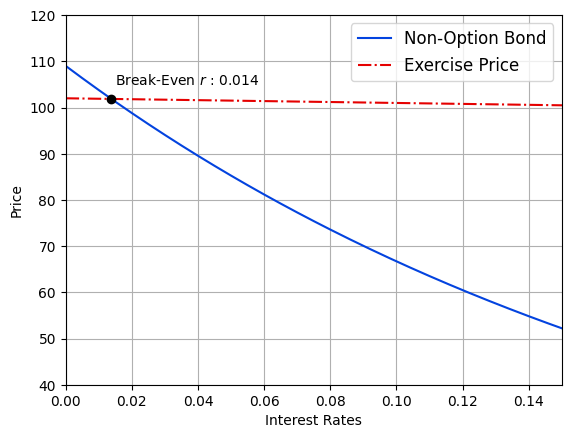
\includegraphics[width=0.5\linewidth]{images/callable_bond}
\end{center}
\end{frame}


%\begin{frame}{Risk Analysis of Callable Bonds}
%	\begin{itemize}
%
%		Callable bonds typically pay a higher coupon or interest rate to investors than non-callable bonds. The companies that issue these products benefit as well. Should the market interest rate fall lower than the rate being paid to the bondholders, the business may call the note. They may then, refinance the debt at a lower interest rate. This flexibility is usually more favorable for the business than using bank-based lending. 
%		
%		However, not every aspect of a callable bond is favorable. An issuer will usually call the bond when interest rates fall. This calling leaves the investor exposed to replacing the investment at a rate that will not return the same level of income. Conversely, when market rates rise, the investor can fall behind when their funds are tied up in a product that pays a lower rate. Finally, companies must offer a higher coupon to attract investors. This higher coupon will increase the overall cost of taking on new projects or expansions.
%	\end{itemize}
%\end{frame}

%\begin{frame}{Risk Analysis of Callable Bonds}
%	\begin{itemize}
%	\item It implies 
%	\begin{equation*}
%		\begin{gathered}
%			NPV_{\text{5y-swap(0)}}=-NPV_{RBS}<0 \\
%			K_1 > K_{\text{5y-swap(0)}}
%		\end{gathered}
%	\end{equation*}
%	??????????????
%	\item Coupons are better than market prevailing rates would have allowed for a fixed rate note.
%	\item After the bond issue if rates go down the bank will call the bond (because, ceteris paribus, it will have a price above 100) as it will not want to pay an higher than market level remuneration for the money it has borrowed from customers,i.e. this is like writing (selling) an option, the option writer gets a premium up front, but has a downside if the option is exercised.
%	\item Conversely if rates go up it will not buy back the bond as in financing itself at a lower than market implied rates.
%	%The call price will usually exceed the par or issue price. In certain cases, mainly in the high-yield debt market, there can be a substantial call premium.
%	%The largest market for callable bonds is that of issues from government sponsored entities. They own many mortgages and mortgage-backed securities. In the U.S., mortgages are usually fixed rate, and can be prepaid early without cost, in contrast to the norms in other countries. If rates go down, many home owners will refinance at a lower rate. As a consequence, the agencies lose assets. By issuing numerous callable bonds, they have a natural hedge, as they can then call their own issues and refinance at a lower rate.
%	%\item It cannot go much above par. The price-yield relation is broken at a certain level.
%	%\item Investors sells an option to the bank for higher (initial) coupons.
%	%\item Customer is long bond, short rates, short option (receiver swaption).
%\end{itemize}
%\end{frame}

%\begin{frame}{Few Useful Math Tricks}
%\renewcommand{\arraystretch}{1.4}
%\begin{table}[bt]
%	\begin{tabular}{|c|c|} \hline
%		rule 1 & $\max(J,K) = K + \max(J-K, 0)$\\ \hline		
%		rule 2 & $\max(J-K,0) = J-K + \max(K-J, 0)$\\ \hline		
%		rule 3 & $\max(\alpha J,K) = \alpha \max(J,\frac{K}{\alpha})$\\ \hline		
%		rule 4 & $\max(\alpha J,K) = K + \alpha\max(J-\frac{K}{\alpha}, 0)$\\ \hline		
%		rule 5 & $\max(J,0) = -\min(-J,0)$\\ \hline		
%		rule 6 & $\begin{aligned}&\min(\max(J-K_{\max}, 0), K_{\min}) =\\ &\max[J-K_{\max},0]-\max[J-K_{\max}-K_{\min},0]\end{aligned}$\\ \hline		
%	\end{tabular}
%\end{table}
%\end{frame}
%
%%A position in options (a situation/ relationship expressed originally as vega) in which any increase in the implied volatility of the underlying asset will generate a profit, even without a move in the underlying asset.
%
%\subsection{Reverse Floater}
%\begin{frame}{Reverse Floater Bond}
%\begin{itemize}
%	\item<1-> Denote with $F(T)$ the short-term rate observed in $T$. We can write the \textcolor{red}{Reverse Floater} coupon in general form as
%	\begin{equation*}
%		\textbf{RF}=\max[0, K-\alpha F(T)] = \underbrace{K-\alpha F(T) + \max[\alpha F(T)-K,0]}_{rule 2}
%	\end{equation*}
%	\item<2-> Previous equation gives the payoff as the sum of a fixed leg of an IRS and a Cap with strike $K$
%\begin{equation}
%	\boxed{\textbf{RF} = \underbrace{K - \alpha F(T)}_{\text{IRS fixed leg}} + \underbrace{\max[\alpha F(T)-K,0]}_{\text{Cap}}}
%\end{equation}
%
%%	\item Which, adding and subtracting $K$ (\emph{rule 1}), and by \emph{rule 5} can be rewritten as
%%	\begin{equation*}
%%		\begin{aligned}
%%		\textbf{RF}&=\max[0, K-\alpha F(T)]=\max[-K,-\alpha F(T)] + K = \\
%%		&= K - \min[K,\alpha F(T)]
%%		\end{aligned}
%%	\end{equation*}
%%	\item Finally \emph{rule 5}, then \emph{rule 1} twice (once with $K$ and another with $\alpha F(T)$) after having added and subtracted $\alpha F(T)$
%%	\begin{equation}
%%		\begin{aligned}
%%			\textbf{RF} &= K - \min[K,\alpha F(T)] = \overbrace{K + \max[-K, -\alpha F(T)]}^{rule 1}\\
%%			&=\underbrace{\max[0, K-\alpha F(T)]}_{rule 5} = \underbrace{K - \alpha F(T) + \max[\alpha F(T)-K,0]}_{rule 2}
%%		\end{aligned}
%%	\label{eq:reverse_floater_payoff}
%%	\end{equation}
%\end{itemize}
%\end{frame}
%
%\begin{frame}{Reverse Floater Bond}
%		\begin{columns}
%			\column{0.45\linewidth}
%		An investor would want to invest in a reverse floater if the benchmark rate is high and she believes the rate will decrease in the future at a faster pace than the forwards indicate.
%			\column{0.4\linewidth}
%				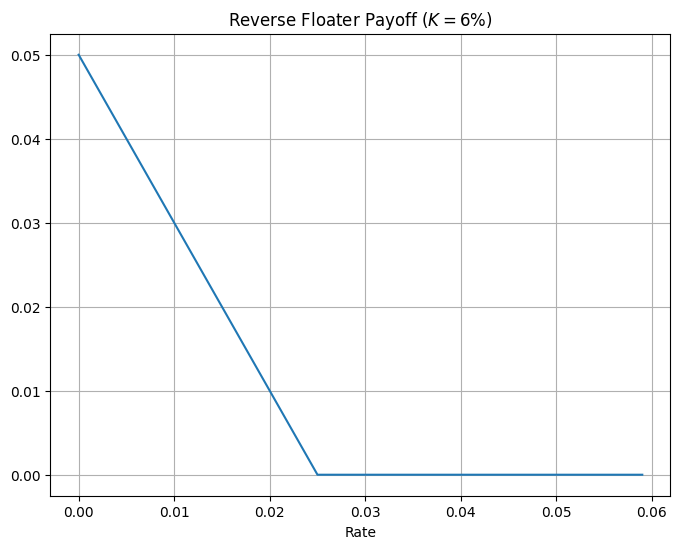
\includegraphics[width=0.8\linewidth]{images/reverse_floater_payoff}
%		\end{columns}
%	\begin{itemize}
%	\item<2-> One can also buy a reverse floater if the rates are low now and believes they stay low, even though the forward contracts are implying an increase. If rates do not change, by holding the reverse floater outperform floating rate notes on the same index.
%	\item<3-> Third if an investor has invested in bonds, and if interest rate falls, she will receive lower returns than expected. In this scenario, inverse floaters in the portfolio provide higher returns.
%	\end{itemize}
%\end{frame}
%
%\begin{frame}{Reverse Floater Bond}
%	\begin{itemize}
%%		\item As with all leveraged investments, inverse floaters introduce significant interest rate risk. 
%		\item Other typical investors are \textbf{long vega}: if $K$ is close to the forward rates, vega is much higher (do you know why ?).
%		\item Such a position means you have a \emph{positive vega exposure}, i.e. take profit from an increase in volatility: 
%		a long call/put option can be used. 
%		\item A \emph{short vega} position instead means you have a negative vega exposure (profit from a decrease in volatility). \item A short call/put option can be used to create a short vega position. 
%		\item High volatility can result in drastic market swings. It typically has a negative correlation to the market, i.e. spiked volatility can be result into downward market velocity.
%	\end{itemize}
%\end{frame}
%
%%\begin{frame}{Reverse Floater Bond}
%%\begin{itemize}
%%	\item 
%%1. Long Vega positions: A long vega position means that you have a positive vega exposure. It is a strategy to profit from an increase in implied volatility. A long call option or a long put option can be used to create a long vega position. 
%%%
%%2. Short Vega positions: A short vega position means that you have a negative vega exposure. It is a strategy to profit from a decrease in implied volatility. A short call option or a short put option can be used to create a short vega position. 
%%
%%	\item Example: when buying an option, the purchaser wants the premium to increase and when selling an option, the seller wants the premium to decrease. Should implied volatility increase, there will be an increase in the option's premium. Inversely, if there is a decrease in implied volatility, there will be a decrease in the option's premium. 
%%	\item Vega changes when there are larger price swings (higher implied volatility) which can be equated to higher uncertainty. Lower implied volatility can be connected to lower uncertainty, which equates to less dramatic swings of the underlying security.
%%	\end{itemize}
%%\end{frame}
%
%\begin{homework}
%\begin{frame}{\textcolor{white}{Homework}}
%\begin{itemize}
%\item[white] Calculate the analytical expressions for:
%\begin{itemize}
%	\item[white] Delta Sensitivity, that is the first derivative of caplet price w.r.t. the forward rate, using the black model to price a generic caplet;
%	\item[white] Vega, that is the first derivative of caplet price w.r.t. the volatility, using the black model to price a generic caplet.
%\end{itemize}
%\end{itemize}
%\end{frame}
%\end{homework}

\end{document}


